% Complete source generated by code/build_article.py.
% Edit the modular source and rebuild, or compile this file directly.
\documentclass[11pt,letterpaper]{article}
\usepackage[T1]{fontenc}
\usepackage{lmodern}
\usepackage[margin=1in,headheight=15pt]{geometry}
\usepackage{amsmath,amssymb,amsthm,mathtools}
\usepackage{microtype,graphicx,booktabs,longtable,array,enumitem,placeins}
\usepackage[dvipsnames]{xcolor}
\usepackage{fancyhdr}
\usepackage[hyphens]{url}
\definecolor{inkblue}{RGB}{25,55,82}
\definecolor{accentteal}{RGB}{0,104,105}
\usepackage[colorlinks=true,linkcolor=inkblue,citecolor=accentteal,urlcolor=inkblue,
 pdfauthor={ProveIt research continuation},
 pdftitle={Sharp Euler Bounds and Uniform Asymptotics in Polylogarithmic Analysis}]{hyperref}
\newtheorem{theorem}{Theorem}[section]
\newtheorem{lemma}[theorem]{Lemma}
\newtheorem{proposition}[theorem]{Proposition}
\newtheorem{corollary}[theorem]{Corollary}
\newtheorem{conjecture}[theorem]{Conjecture}
\theoremstyle{definition}
\newtheorem{definition}[theorem]{Definition}
\theoremstyle{remark}
\newtheorem{remark}[theorem]{Remark}
\DeclareMathOperator{\Li}{Li}
\DeclareMathOperator{\mesh}{mesh}
\DeclareMathOperator{\diag}{diag}
\DeclareMathOperator{\rank}{rank}
\newcommand{\sourcecommit}{\texttt{3447bc59b78d138a7f0d536b66ac6e5cc5d5e49f}}
\newcommand{\code}[1]{\nolinkurl{#1}}
\newcolumntype{P}[1]{>{\raggedright\arraybackslash}p{#1}}
\setlength{\emergencystretch}{2em}
\setlength{\parskip}{3pt}
\setlist{itemsep=3pt,topsep=5pt}
\allowdisplaybreaks[2]
\pagestyle{fancy}
\fancyhf{}
\fancyhead[L]{\small\color{inkblue}Polylogarithmic analysis: research continuation}
\fancyhead[R]{\small October 2026}
\fancyfoot[C]{\thepage}
\renewcommand{\headrulewidth}{0.3pt}
\title{\color{inkblue}\bfseries Sharp Euler Bounds and Uniform Asymptotics\\[3pt]
 in Polylogarithmic Analysis\\[8pt]
 \large\normalfont Reflected moments, Lerch zeros, and integral shuffle lattices}
\author{A research continuation for the ProveIt project}
\date{10 October 2026}

\begin{document}

% ===== sections/01_introduction.tex =====
\maketitle
\begin{abstract}
We continue the polylogarithm manuscript at the pinned repository revision
identified in Appendix~\ref{app:provenance}. Four proof developments are obtained. First, an elementary
multiplicative-increment inequality controls every Gaussian Euler remainder
at arbitrary positive real orders. It identifies the least universal
constant as $C_*=\max_{b>0}\{\beta(b)+2^{-b}\eta(b)\}$, and exact rational
certificates enclose its unique maximizer and its value. Second, the
coordinate $y=\log\Gamma(x)$ gives an all-orders expansion of reflected
log-gamma moments uniformly for every ratio of their two nonnegative
exponents, as the larger exponent tends to infinity. Third, an explicit
Appell-root separation bound and a logarithmic variation estimate for
the Lerch kernel yield an effective saturation threshold and simultaneous
zero locations when the Laurent index grows with the derivative order.
Fourth, a central-factorial identity integrally diagonalizes the odd-weight
shuffle minor, giving its cokernel, Smith factors, field ranks, and optimal
common inverse denominator. Weight-eleven and weight-thirteen Gaussian
relations are recorded as conjectures with exact finite proximity
certificates. Established source results, new proofs, finite certificates,
numerical diagnostics, and unresolved claims are distinguished throughout.
\end{abstract}

\tableofcontents
\clearpage

\section{Scope, prior results, and the new claims}
\label{sec:introduction}

The starting point is the 375-page manuscript in
\code{Analysis/Polylogarithms/docs/manuscript}, together with the relevant
reports already present in the same repository at the pinned revision
\cite{repo}. The version matters: the $S_4$ identity, several Gaussian
reductions, and the rational relation ranks were already proved there.
Repeating those results as new conjecture resolutions would misstate the
state of the project. The existing $S_6$ special-value conjecture remains
unresolved by the present work.

The objective is to close specific gaps in the current programme and
provide reusable structural results. The universal Euler question has a
particularly direct answer: the existing Gaussian-axis maximum really is
the sharp error constant, once a new comparison is proved for \emph{all}
Euler indices. The reflected-moment question requires a different kind of
step. Separate fixed-exponent and bounded-ratio asymptotics do not justify
substitution of an unbounded exponent ratio. A change of coordinate and
an appropriate placement of the Jacobian in the phase give uniform
derivative and tail estimates on the full parameter range.

The zero problem has a similar obstruction to naive extrapolation. A
fixed-index expansion on a compact scale does not control the extreme
roots when the index grows. Our proof works with relative polynomial
errors on the logarithmic coordinate and with a scale-independent
positive-weight inequality. The resulting threshold is intentionally
conservative, but it is explicit, uniform in the Lerch parameter, and
applies to every positive root at once.

The algebraic part is separate from those analytic estimates. A rational
rank says that a coordinate system works over $\mathbb Q$. Integral
diagonalization additionally determines its torsion and all primes of
coordinate failure. The matrix is closely related to Zagier's double-zeta
matrix \cite{Zagier,Ma,MaTeo}; this connection is credited rather than
treated as evidence of new priority. The proof given here is constructive
and supplies the integral information directly in the manuscript's
shuffle coordinates.

\subsection{A claim and dependency map}

\begin{longtable}{@{}P{0.19\textwidth}P{0.46\textwidth}P{0.29\textwidth}@{}}
\toprule
Result & New conclusion & Inherited input or limitation\\
\midrule
\endhead
Euler remainder & The least constant uniform in $a,b>0$ and $N\ge1$ is
$C_*$; $C(b)$ is optimal at each fixed $b$. & The source's unique-axis-maximum
theorem identifies the sole maximizing $b_*$.\\
Exact maximum & Rational enclosures for $b_*$ and $C_*$, and the useful
budget $C_*<57/50$. & Finite exact arithmetic plus the proved qualitative
unimodality.\\
Reflected moments & All fixed asymptotic orders, uniformly for
$0\le m\le n$ as $n\to\infty$. & The previously certified global
log-gamma slope inequality; no exponentially small error is claimed.\\
Lerch zeros & Explicit $K_n$ and relative locations uniform in every
branch and $0\le\rho\le1$; a growing-index regime follows. & The
standard positive integral and Laplace zero-count principle, reviewed
in the proof. The threshold is sufficient, not sharp.\\
Shuffle lattice & Integral equivalence to
$\diag(1,3,\ldots,2m-1)$, hence the full arithmetic of the minor. & A
formal shuffle presentation; no period-independence conclusion.\\
Gaussian candidates & Frozen $S_{10}$ and $S_{12}$ formulas with exact
normalized residual bounds below $10^{-650}$. & They remain conjectures;
the residual intervals contain zero.\\
\bottomrule
\end{longtable}

All main analytic and algebraic statements are proved in ordinary
mathematical language. The exact certificates have explicitly narrower
roles: they certify constant brackets, check a pre-existing slope
inequality, or establish finite residual enclosures. They are not a
substitute for an identity proof, and no Lean formalization is claimed.

\subsection{Notation and branch conventions}

We use decreasing nested indices:
\[
 \Li_{a,b}(z,1)=\sum_{n>r\ge1}\frac{z^n}{n^a r^b},\qquad
 H_n^{(b)}=\sum_{r=1}^n r^{-b},\qquad H_n=H_n^{(1)}.
\]
The double family $F_{a,b}(z)$ always denotes this one-variable
specialization, initially in $|z|<1$. Real-order values at $i$ mean
the principal analytic continuation. At some small real orders the
ordinary boundary series does not converge, which does not affect the
finite Euler transforms or their proved limit. All gamma powers in real
integrals use positive real bases. The Dirichlet beta and eta functions
are denoted by $\beta$ and $\eta$; Euler's constant is $\gamma$.

In the moment section only, $F(x)=-\psi(x)$ is a positive real function;
the argument and absence of subscripts distinguish it from the double
polylogarithm. In the Lerch section $F_{n,k}^\rho$ is a signed normalization
of a parameter derivative, defined explicitly there. These local
notations follow the corresponding source problems and are not
identifications of different functions.

\subsection{Reading the computational evidence}

The accompanying archive contains the full LaTeX source, compiled PDF,
reusable section fragments, exact verifiers, frozen candidates, interval
certificates, numerical diagnostics, figure-generation code, a provenance
record, and integration notes. Each computational result says what it
establishes. For example, the equality $UMV=D$ is exact integer algebra;
an enclosure $|R|<10^{-650}$ is a finite analytic error statement; and
a plot of asymptotic errors is a floating-point diagnostic. None of these
labels is used interchangeably.

The original log-gamma moment problem and its fixed-order asymptotics
have substantial prior literature \cite{Amdeberhan,Bailey}. Our contribution
is the unrestricted-ratio theorem, rather than the definition or first
asymptotic observation. Likewise, the classical Laplace and gamma-series
tools used below are standard \cite{DLMFLaplace,DLMFGamma}; uniformity in
the present parameter domain is proved explicitly.

% ===== sections/02_euler.tex =====
% Research continuation at source commit 3447bc59b78d138a7f0d536b66ac6e5cc5d5e49f.
% New result: the global real-order Euler constant is the existing axis maximum.
% This is a self-contained section fragment, not a standalone document.

\section{The sharp universal Euler constant at all positive real orders}
\label{newEuler:sec}

Write
\[
 c_n=\frac{H_{n-1}^{(b)}}{n^a},\qquad
 F_{a,b}(z)=\sum_{n\ge1}c_nz^n,
 \qquad a\ge0,\quad b>0,
\]
where values away from the disk use the principal continuation to
$\mathbb C\setminus[1,\infty)$. Set
\[
 g_{a,b}=\operatorname{Im}F_{a,b}(i),\quad
 d_j=\sum_{k=0}^j(-1)^k\binom jk c_{2k+1},\quad
 E_N=\sum_{j=0}^{N-1}2^{-j-1}d_j\quad(N\ge1).
\]
The manuscript proves one-sided Euler convergence throughout this domain,
but explicitly leaves a universal error constant in the supercritical
fractional-order region open. The Gaussian maximum established there
controls only the first Euler remainder. The following scalar inequality
supplies the missing comparison for every later remainder.

\subsection{An elementary comparison of scalar Euler kernels}

For an integer $N\ge1$ put
\[
 \Phi_N(t)=\frac{(1-t)^N}{1+t}\qquad(0\le t\le1).
\]
\begin{lemma}[Uniform multiplicative-increment bound]
\label{newEuler:lem:scalar}
For every integer $N\ge1$ and $q,t\in[0,1]$,
\begin{equation}\label{newEuler:eq:scalar}
 0\le\Phi_N(qt)-\Phi_N(t)\le\frac{1-q}{1+q}.
\end{equation}
The upper inequality is strict when $0<q<1$ and $0<t<1$.
For $0<q<1$ and $t=1$, equality in the upper inequality occurs
exactly when $N=1$.
\end{lemma}
\begin{proof}
The first inequality follows from the decrease of $\Phi_N$. For the
second define $f_N(u)=u^N/(2-u)$ on $[0,1]$ and set
$A=1-qt$, $B=1-t$, and $p=A+B$. The cases $q=1$ or $t=0$ are
immediate, so suppose $A>B$. The desired inequality is equivalent to
\begin{equation}\label{newEuler:eq:divided}
 \frac{f_N(A)-f_N(B)}{A-B}\le\frac1{2-A-B}.
\end{equation}
The exceptional case $A=B=1$ has already been excluded.

The derivative $f_N'$ is strictly convex on $(0,1)$: expand
\[
 f_N(u)=\sum_{j=0}^{\infty}\frac{u^{N+j}}{2^{j+1}}
\]
and differentiate three times; the result is strictly positive for
$0<u<1$. The average of a convex function over a centered interval
is nondecreasing as its length increases. Explicitly, if
$h\mapsto (2h)^{-1}\int_{c-h}^{c+h}g(v)\,dv$ is differentiated,
the result is nonnegative by the trapezoid bound for a convex $g$.
It is strictly positive for a strictly convex $g$ and a nondegenerate
interval. Applying this to $g=f_N'$ shows that the divided difference
on the left of \eqref{newEuler:eq:divided}, at fixed sum $p$, increases
as the endpoints move apart.

If $p\le1$, enlarge $[B,A]$ to $[0,p]$. Then
\[
 \frac{f_N(A)-f_N(B)}{A-B}
 \le\frac{f_N(p)-f_N(0)}p
 =\frac{p^{N-1}}{2-p}\le\frac1{2-p}.
\]
If $p\ge1$, enlarge it instead to $[p-1,1]$. Since $f_N(1)=1$
and $f_N(p-1)\ge0$,
\[
 \frac{f_N(A)-f_N(B)}{A-B}
 \le\frac{1-f_N(p-1)}{2-p}\le\frac1{2-p}.
\]
When $0<t<1$ and $0<q<1$, both original endpoints are interior
to $[0,1]$, so the interval is strictly enlarged in the appropriate
case and strict convexity gives a strict inequality. At $t=1$ the
original difference equals $(1-q)^N/(1+q)$, proving the equality
statement. The endpoint $q=0$ follows directly from
$\Phi_N(0)-\Phi_N(t)=1-\Phi_N(t)\le1$.
\end{proof}

\subsection{A probability formula for every Euler remainder}

For $a>0$ let $S\sim\operatorname{Gamma}(a,1)$ and
$T\sim\operatorname{Gamma}(b,1)$ be independent, and set
$X=e^{-S}$, $V=e^{-T}$. When $a=0$, define $S=0$, $X=1$
deterministically. A finite geometric sum and the Gamma integral give
\begin{equation}\label{newEuler:eq:moments}
 c_n=\mathbb E\!\left[
       \frac{X^{n-1}-(XV)^{n-1}}{1-V}\right]\quad(n\ge1).
\end{equation}
Indeed the expectation factors as
$n^{-a}\sum_{k=0}^{n-2}(k+1)^{-b}$, including the empty sum at
$n=1$. For $a>0$ this is the existing positive double kernel in
probability coordinates; no signed moment measure is required.

\begin{theorem}[Universal one-sided remainder identity and domination]
\label{newEuler:thm:domination}
For every $a\ge0$, $b>0$ and integer $N\ge1$, the Euler series
converges absolutely, $d_0=0$, $d_j<0$ for $j\ge1$, and
$E_N$ decreases strictly to $g_{a,b}$. More precisely, with
$R_N(a,b)=2^N(E_N-g_{a,b})$,
\begin{equation}\label{newEuler:eq:R}
 R_N(a,b)=\mathbb E\!\left[
 \frac{\Phi_N(X^2V^2)-\Phi_N(X^2)}{1-V}\right]>0.
\end{equation}
Define
\begin{equation}\label{newEuler:eq:C}
 C(b)=\beta(b)+2^{-b}\eta(b)
     =\mathbb E\!\left[\frac{1+V}{1+V^2}\right],
\end{equation}
where $\beta$ is the Dirichlet beta function and
$\eta(b)=\sum_{n\ge1}(-1)^{n-1}n^{-b}$. Then
\begin{equation}\label{newEuler:eq:fixedb}
 R_N(a,b)<C(b)\qquad(a>0,b>0,N\ge1).
\end{equation}
At $a=0$, the same estimate is non-strict, and equality holds exactly
when $N=1$. In addition, $R_N(a,b)\to0$ as $N\to\infty$ for every
fixed pair in the stated domain.
\end{theorem}
\begin{proof}
Applying a finite binomial sum to \eqref{newEuler:eq:moments} gives
\[
 d_j=\mathbb E\!\left[
  \frac{(1-X^2)^j-(1-X^2V^2)^j}{1-V}\right].
\]
This is zero for $j=0$ and strictly negative for $j\ge1$. Every
fixed integrand is bounded by $2j$, by the mean-value theorem, so
all displayed finite expectations are legitimate.

The positive double-kernel continuation at $i$ gives
\begin{equation}\label{newEuler:eq:Gaussian}
 -g_{a,b}=\mathbb E\!\left[
 \frac{X^2(1+V)}{(1+X^2)(1+X^2V^2)}\right]>0.
\end{equation}
This remains valid on the axis $a=0$ from
$F_{0,b}(z)=z\operatorname{Li}_b(z)/(1-z)$.
Alternatively, expanding the two denominators in the disk gives
\eqref{newEuler:eq:moments}, and dominated continuation gives
\eqref{newEuler:eq:Gaussian}.

Tonelli's theorem, applied to the nonnegative functions $-d_j$, permits
summing the infinite Euler series before proving its finiteness. The
geometric sum gives
\[
 \sum_{j\ge0}\frac{-d_j}{2^{j+1}}
 =\mathbb E\!\left[
  \frac{(1+X^2V^2)^{-1}-(1+X^2)^{-1}}{1-V}\right]
 =-g_{a,b}<\infty.
\]
Thus the Euler series is absolutely convergent and its sum is $g$.
The same geometric summation beginning at $j=N$ proves
\eqref{newEuler:eq:R}. The positivity and strict decrease of $E_N$
follow from the strict signs of $d_j$ for $j\ge1$.

Apply Lemma~\ref{newEuler:lem:scalar} with $t=X^2$ and $q=V^2$.
It gives the pointwise domination
\[
 0<\frac{\Phi_N(X^2V^2)-\Phi_N(X^2)}{1-V}
 \le\frac{1-V^2}{(1+V^2)(1-V)}
 =\frac{1+V}{1+V^2}.
\]
The upper inequality is strict almost surely for $a>0$. On the axis
it is equality precisely at $N=1$. Taking expectations proves
\eqref{newEuler:eq:fixedb}. To identify $C(b)$, write the density
of $V$ as $(-\log v)^{b-1}\,dv/\Gamma(b)$ on $(0,1)$, and
integrate the even and odd geometric series for $(1+v)/(1+v^2)$.
Their partial sums are bounded uniformly, justifying dominated
convergence; the resulting alternating Dirichlet series are exactly
$\beta(b)+2^{-b}\eta(b)$ for every $b>0$.

For every $0<X\le1$ and $0<V<1$, both powers in the numerator of
\eqref{newEuler:eq:R} tend to zero as $N\to\infty$.
The same integrable domination, independent of $N$, proves $R_N\to0$.
\end{proof}

\subsection{The least constant uniform in both real orders}

The preceding manuscript already proves that $C$ has exactly one
stationary point $b_*$, a nondegenerate global maximum, with
$1<b_*<2$. Denote its value by
\[
 C_*:=C(b_*)=\max_{b>0}\{\beta(b)+2^{-b}\eta(b)\}.
\]
Its reported numerical diagnostics are
\[
 b_*\approx1.30221658710124120959,\qquad
 C_*\approx1.13656110333950956095;
\]
these decimal values are not needed for the theorem. The existing exact
bounds $227/200<C_*<(1+\sqrt2)/2$ may be retained.

\begin{corollary}[Sharp universal real-order Euler bound]
\label{newEuler:cor:sharp}
For all $a,b>0$ and all integers $N\ge1$,
\begin{equation}\label{newEuler:eq:universal}
 E_N-C_*2^{-N}<g_{a,b}<E_N.
\end{equation}
The number $C_*$ is the least constant for which this assertion holds
uniformly over the entire positive quadrant. With $a=0$ included,
$0<R_N\le C_*$, and equality occurs exactly at
$(a,b,N)=(0,b_*,1)$. For each fixed $b>0$, the least constant uniform
in $a>0$ and $N\ge1$ is $C(b)$.
\end{corollary}
\begin{proof}
The upper bound follows from \eqref{newEuler:eq:fixedb} and
$C(b)\le C_*$. For sharpness, take $N=1$, for which $E_1=0$ and
$R_1=-2g$. As $a\downarrow0$, $S\sim\operatorname{Gamma}(a,1)$
tends to zero in probability (its mean is $a$), so $X\to1$.
The bounded integrand in \eqref{newEuler:eq:Gaussian}, or the
pointwise domination already proved, gives
\[
 \lim_{a\downarrow0}R_1(a,b)=C(b).
\]
Taking $b=b_*$ shows that every smaller universal constant fails for
some positive $a$. The same argument at a fixed $b$ proves its
claimed sharp constant. Strictness and the sole equality case on the
closed outer-order axis follow from the theorem and the uniqueness
of the maximum of $C$.
\end{proof}

The derivative of $(1+v)/(1+v^2)$ is
$(1-2v-v^2)/(1+v^2)^2$, so its maximum on $[0,1]$ is
$(1+\sqrt2)/2<5/4$, attained at $v=\sqrt2-1$.
Theorem~\ref{newEuler:thm:domination} therefore supplies the
self-contained budget $R_N(a,b)<5/4$ throughout the domain.
The explicit algebraic choice $(1+\sqrt2)/2$ gives an immediate
universal enclosure without optimization in $b$.
The established constant one for $a\ge1$ remains sharper on that
restricted region. The new result resolves precisely the outstanding
supercritical fractional-order question; it does not assert that the
scaled errors are monotone in $N$ there, nor that the fixed-pair
constant equals $-2g$ there.

\subsection{A convenient rational certificate for the universal constant}
\begin{proposition}[An elementary rational error budget]
\label{newEuler:prop:rational}
The sharp universal constant satisfies $C_*<57/50$. Consequently
\[
 E_N-\frac{57}{50}\,2^{-N}<g_{a,b}<E_N
 \qquad(a,b>0,\ N\ge1).
\]
\end{proposition}
\begin{proof}
The existing axis-maximum theorem gives $b_*\in(1,2)$. By its positive
Mellin representation, $M(b)=\Gamma(b)C(b)$ is log-convex. Also
\[
 (\log\Gamma)''(b)=\sum_{j\ge0}\frac1{(j+b)^2}
 \le\frac{\pi^2}{6}<\frac53\qquad(1\le b\le2).
\]
On an interval $[u,u+h]\subset[1,2]$, the error of linear
interpolation of $\log\Gamma$ is therefore at most $5h^2/24$.
Combining this with the convexity inequality for $\log M$ yields
\[
 C(b)\le\max\{C(u),C(u+h)\}\exp(5h^2/24).
\]
The accompanying exact standard-library verifier
\texttt{certify\_rational\_euler\_constant.py} proves
\[
 C(k/10)<\frac{1137}{1000}\qquad(k=10,11,\ldots,20).
\]
It uses 80 terms of the axis Euler enclosure with error
budget $5/4$, which follows directly from the scalar domination above
and was also available in the preceding manuscript. Every $n^{-k/10}$ is enclosed on a $2^{-160}$ grid
by integer inequalities: if
$r=\lfloor (2^{1600}/n^k)^{1/10}\rfloor$, then
$r^{10}n^k\le2^{1600}<(r+1)^{10}n^k$. All subsequent operations
are exact rational arithmetic. The full rational intervals are saved
in \texttt{rational\_euler\_constant\_certificate.json}; none of the
displayed decimal diagnostics is used for a sign decision.
Taking $h=1/10$ gives
\[
 C_*<\frac{1137}{1000}e^{1/480}
 <\frac{1137}{1000}\frac{480}{479}
 =\frac{13644}{11975}<\frac{57}{50}.
\]
The exponential inequality follows from its positive series and
$e^x<(1-x)^{-1}$ for $0<x<1$.
\end{proof}

\begin{proposition}[A narrow exact enclosure of the sharp constant]
\label{newEuler:prop:narrow}
The unique maximizer and its value satisfy
\[
 1.3022165871012412095923717014
 <b_*<1.3022165871012412095923717017,
\]
\[
 \begin{gathered}
 1.136561103339509560952586375779942387681723540765044951\\
 <C_*<\\
 1.136561103339509560952586375779942387681723540765044952.
 \end{gathered}
\]
These are exact rational enclosures, not estimates from a
floating-point stationary-point calculation.
\end{proposition}
\begin{proof}
Let $L,R$ be the displayed endpoints for $b_*$, and put
$c=1.30221658710124120959237170155$. The standard-library verifier
\texttt{certify\_axis\_maximum.py} encloses $C(L)$, $C(c)$ and
$C(R)$ by exact rational intervals and proves
\[
 C(c)>C(L),\qquad C(c)>C(R).
\]
The previously proved strict unimodality implies $L<b_*<R$.

Here are all arithmetic ingredients of that finite certificate.
The computation uses 224 axis Euler terms, with the self-contained
error budget $5/4$ proved above. To enclose $n^{-b}$ for rational $b$, write
$n=2^k r$, $1\le r<2$, and use
\[
 \log n=k\log2+2\sum_{j=0}^{127}\frac{z^{2j+1}}{2j+1}
             +\mathcal R,\qquad z=\frac{r-1}{r+1},
 \quad 0\le\mathcal R\le\frac{2z^{257}}{257(1-z^2)}.
\]
The same formula with $z=1/3$ encloses $\log2$. For each resulting
$0\le x=b\log n<8$, sum the positive exponential series through
$x^{200}/200!$, with tail bounded by
\[
 \frac{x^{201}}{201!}\frac1{1-x/202},
\]
and reciprocate the interval. Every operation is rounded outwards
on the dyadic grid $2^{-384}$. All sum weights and error budgets
are exact rational numbers. The complete rational intervals, along
with the strict comparisons above, are recorded in
\texttt{axis\_maximum\_certificate.json}.

For the upper enclosure on the maximum, the interpolation argument
in Proposition~\ref{newEuler:prop:rational} gives, with
$\delta=5(R-L)^2/24$,
\[
 C(c)\le C_*\le\max\{C(L),C(R)\}e^{\delta}
 <\frac{\max\{C(L),C(R)\}}{1-\delta}.
\]
Applying the rational lower endpoint for $C(c)$ and the two rational upper
endpoints at $L,R$, then rounding the final bounds outwards to
54 decimal places, proves the displayed enclosure.
\end{proof}

% ===== sections/03_moments.tex =====
\section{A uniform saddle expansion for all reflected exponent ratios}
\label{sec:all-ratios}

Let $f(x)=\log\Gamma(x)$ and $F(x)=-\psi(x)$ on $0<x<1$.
Both functions are positive. For real $n,m\ge0$ put
\[
 M_{n,m}=\int_0^1 f(x)^n f(1-x)^m\,dx.
\]
Reflection gives $M_{n,m}=M_{m,n}$, so it is enough to consider
$n\ge m$. The previously proved compact-ratio theorem does not provide a uniform
estimate on the entire range $n/m\ge1$: its saddle in the $x$ coordinate
approaches an endpoint. The following construction uses a coordinate
and a phase which remain uniformly suitable in that limit.

\subsection{The inverse coordinate and the one needed inherited lemma}

Write $x(y)$ for the decreasing inverse of $f$, and define, for $y>0$,
\begin{equation}\label{eq:ratio-definitions}
 q(y)=f(1-x(y)),\qquad
 d(y)=\frac{e^y}{F(x(y))},\qquad
 r(y)=-\frac{yq'(y)}{q(y)}.
\end{equation}
Thus $q$ is positive and decreasing, while $d$ is positive. Direct
differentiation gives
\begin{equation}\label{eq:ratio-J}
 r(y)=\frac{1}{J(x(y))},\qquad
 J(x)=\frac{F(x)f(1-x)}{F(1-x)f(x)}.
\end{equation}
We use the following established result from the pinned repository.

\begin{lemma}[Inherited global slope inequality]\label{lem:inherited-J}
The function $J$ is an increasing real-analytic bijection
$(0,1)\longrightarrow(0,\infty)$, and
$J'(x)/J(x)>176/225$. Consequently $r$ is an increasing
real-analytic bijection $(0,\infty)\longrightarrow(0,\infty)$,
with $r'(y)>0$.
\end{lemma}

The source is the theorem entitled ``Certified global log-gamma slope
ratio'' in the report \emph{Uniform Transitions and Integral Structures},
at the revision recorded in the provenance appendix. This is an inherited
theorem, not a new assertion of this article. Its proof treats the
endpoints analytically and proves the compact inequality with 256 exact
dyadic interval computations. The dependency is included with its source
attribution and freshly replayed in this package. To verify the consequence,
differentiate \eqref{eq:ratio-J}, using $x'(y)=-1/F(x(y))$.

We also need elementary quantitative information at infinity. Put
\[
 c=\frac{\zeta(2)}{2\gamma}-\gamma>0.
\]
The inverse-function theorem applied to
$x=e^{-y}\Gamma(1+x)$ and the convergent log-gamma series yield
\begin{align}
 x(y)&=e^{-y}-\gamma e^{-2y}+O(e^{-3y}),\notag\\
 q(y)&=\gamma e^{-y}\{1+c e^{-y}+O(e^{-2y})\},\label{eq:inverse-infinity}\\
 d(y)&=1-2\gamma e^{-y}+O(e^{-2y}),\notag\\
 r(y)&=y\{1+c e^{-y}+O(e^{-2y})\}.\notag
\end{align}
Every fixed number of derivatives may be taken in these expansions.
More precisely, the correction functions in $q(y)e^y/\gamma$ and
$d(y)$ are analytic functions of $e^{-y}$ near zero. In particular,
for each fixed $j\ge2$,
\begin{equation}\label{eq:derivative-bounds}
 (\log q)^{(j)}(y)=O_j(e^{-y}),\qquad
 d^{(j)}(y)=O_j(e^{-y}),\qquad r'(y)\longrightarrow1.
\end{equation}
The statement for $d^{(j)}$ also holds for $j=1$.
Near zero, $x(y)=1-y/\gamma+O(y^2)$, so
$q(y)=\log(\gamma/y)+o(1)$ and $d(y)\to1/\gamma$.
Consequently $d$ has positive finite global upper and lower bounds.

\subsection{The all-ratio theorem}

Define
\begin{equation}\label{eq:uniform-phase}
 \Phi_{n,m}(y)=n\log y+m\log q(y)-y.
\end{equation}
The last term incorporates the exponential part of the Jacobian; keeping
it in the phase is essential when $m$ is small. The exact change of
variables is
\begin{equation}\label{eq:exact-y-moment}
 M_{n,m}=\int_0^\infty e^{\Phi_{n,m}(y)}d(y)\,dy.
\end{equation}

\begin{theorem}[Uniform expansion without a ratio restriction]
\label{thm:all-ratio}
For every real $n>0$ and $m\ge0$ there is exactly one positive solution
$s=s(n,m)$ of
\begin{equation}\label{eq:uniform-saddle}
 n=s+m r(s).
\end{equation}
It is the unique global maximizer of \eqref{eq:uniform-phase}, and
\[
 H=-\Phi_{n,m}''(s)=\frac{1+m r'(s)}{s}>0.
\]
For each fixed integer $K\ge0$, as $n\to\infty$,
\begin{equation}\label{eq:uniform-moment-expansion}
 M_{n,m}=e^{\Phi_{n,m}(s)}d(s)\sqrt{\frac{2\pi}{H}}
 \left\{\sum_{j=0}^{K}\frac{L_j(n,m)}{n^j}
                  +O_K(n^{-K-1})\right\},
 \qquad 0\le m\le n.
\end{equation}
The error constant is independent of $m$, and each coefficient
$L_j(n,m)$ is bounded on $n\ge2$, $0\le m\le n$.
Here $L_0=1$. With derivatives evaluated at $s$,
\begin{equation}\label{eq:uniform-first}
 \frac{L_1}{n}=
 \frac{d''}{2dH}
 +\frac{d'\Phi^{(3)}}{2dH^2}
 +\frac{\Phi^{(4)}}{8H^2}
 +\frac{5(\Phi^{(3)})^2}{24H^3}.
\end{equation}
The leading factor can equivalently be written
\begin{equation}\label{eq:uniform-leading-x}
 \frac{s^n q(s)^m}{F(x(s))}
       \sqrt{\frac{2\pi s}{1+m r'(s)}}.
\end{equation}
Thus reflection supplies an expansion for every pair $n,m\ge0$ as
$\max(n,m)\to\infty$.
\end{theorem}

\begin{proof}
First,
\[
 \Phi_{n,m}'(y)=\frac{n-y-mr(y)}{y}.
\]
The function $h_m(y)=y+mr(y)$ increases strictly from zero to infinity.
The derivative of the phase is therefore positive before its unique
zero and negative afterwards. At that zero its second derivative is
$-h_m'(s)/s$, proving the existence, uniqueness and curvature assertions.

The issue is uniformity, rather than this stationary calculation.
Choose $s_0>0$ so small that $s_0<1/2$ and $r(s_0)<1/2$.
For $n\ge2$, $0\le m\le n$, the saddle equation precludes $s\le s_0$:
otherwise $n=s+mr(s)<1/2+n/2<n$. Thus $s>s_0$ uniformly.
On $[s_0/2,\infty)$, positivity, continuity and
\eqref{eq:inverse-infinity} give constants $c_0,C_0,c_1,C_1>0$ such that
\begin{equation}\label{eq:uniform-comparability}
 c_0\le r(y)/y\le C_0,\qquad c_1\le r'(y)\le C_1.
\end{equation}
It follows from the saddle equation that
\[
 n\asymp(m+1)s,\qquad H\asymp n/s^2,
\]
with absolute constants throughout the stated parameter range.

For $y,s\ge s_0/2$, the mean-value estimate
$h_m'\ge c(m+1)$ gives a global phase bound. Integrating
$\Phi'=(h_m(s)-h_m(y))/y$ on either side of $s$ yields
\begin{equation}\label{eq:uniform-gap}
 \Phi(y)-\Phi(s)
 \le-c_2n\{y/s-1-\log(y/s)\}
 \qquad(y\ge s_0/2)
\end{equation}
for one constant $c_2>0$. This calculation has the same sign on both
sides: if $y<s$, integrate the positive derivative from $y$ to $s$.
The portion $0<y<s_0/2$ is also harmless. The phase is increasing there,
so its integral is at most a constant times
$e^{\Phi(s_0/2)}$. In \eqref{eq:uniform-gap},
$(s_0/2)/s\le1/2$; hence this contribution is exponentially small
relative to $e^{\Phi(s)}s/\sqrt n$.

Now put $u=y/s$ and
\[
 \varphi(u)=\frac{\Phi(su)-\Phi(s)}n,
 \qquad b(u)=\frac{d(su)}{d(s)},
 \qquad A=-\varphi''(1)=\frac{s(1+mr'(s))}{n}.
\]
The number $A$ is bounded above and bounded away from zero. Every fixed
derivative of $\varphi$ and $b$ is bounded uniformly on $1/2\le u\le3/2$.
For example, for $j\ge2$,
\[
 \varphi^{(j)}(u)
 =(-1)^{j-1}(j-1)!u^{-j}
   +\frac{m}{n}s^j(\log q)^{(j)}(su),
\]
and the second term is bounded by \eqref{eq:derivative-bounds}, compactness
on bounded $s$, and $\sup_{s\ge s_0}s^j e^{-s/2}<\infty$.
The same argument bounds the derivatives of $b$.

These estimates give a parameter-independent neighborhood of $u=1$
on which $\varphi(u)\le-c_3(u-1)^2$. Outside that neighborhood,
\eqref{eq:uniform-gap} gives an exponentially small integrable tail.
For clarity, integrability on the unbounded part follows from the linear
growth of $u-1-\log u$ as $u\to\infty$; near zero it follows from its
growth like $-\log u$.

Here is a more explicit remainder argument. Put $u=1+v/\sqrt n$ and
first restrict $|v|\le n^\epsilon$, with a positive $\epsilon$ chosen
sufficiently small for the desired fixed order $K$. On this interval,
the cubic and all higher phase terms are uniformly small relative to
the quadratic term. Taylor-expand the amplitude and the exponential
of those higher terms, retaining all powers through $n^{-K-1/2}$.
Using, for example, phase and amplitude derivatives through order
$4K+8$ and then decreasing $\epsilon$ if necessary bounds the omitted
integrand by $C_K n^{-K-1}(1+|v|^{D_K})e^{-c_4v^2}$ for a fixed
integer $D_K$. The uniform derivative bounds established above justify
these Taylor remainders. The region $|v|>n^\epsilon$ within the common
neighborhood is smaller than every power of $n^{-1}$ by the quadratic
gap; the preceding global bound handles the rest. All retained odd
powers integrate to zero after extension to the whole real line,
whose error is again smaller than every power. This proves the stated
uniform $O_K(n^{-K-1})$ normalized remainder. Boundedness of the
coefficient functions follows from the derivative bounds and the
lower bound on $A$.

For an explicit finite prescription, set
$\kappa_j=s^j\Phi^{(j)}(s)/n$ and
$b_j=s^j d^{(j)}(s)/d(s)$. If $Z$ is centered Gaussian of variance
$A^{-1}$, then $L_j$ is the coefficient of $t^{2j}$ in
\begin{equation}\label{eq:uniform-coefficient-rule}
 \mathbb E\left[
 \left(\sum_{r\ge0}\frac{b_r Z^r t^r}{r!}\right)
 \exp\left\{\sum_{r\ge3}\frac{\kappa_rZ^r t^{r-2}}{r!}\right\}
 \right].
\end{equation}
Each coefficient uses finitely many terms. The degree-two coefficient
gives \eqref{eq:uniform-first}; substitution of $d=e^s/F(x(s))$
gives \eqref{eq:uniform-leading-x}.
\end{proof}

\subsection{What uniformity does and does not imply}

The theorem includes balanced moments, fixed positive exponent ratios,
the logarithmic transition, fixed reflected exponent, and the axis $m=0$.
No lower bound on $m$ is needed. If $m$ is fixed, then
\[
 s=\frac{n}{m+1}+O_m(ne^{-n/(m+1)}),
\]
and the leading factor in \eqref{eq:uniform-moment-expansion} reduces to
the leading Stirling approximation of
$\gamma^m\Gamma(n+1)/(m+1)^{n+1}$. In the ideal limiting kernel
$q(y)=\gamma e^{-y}$, $d(y)=1$, the first coefficient is exactly
$L_1=1/12$, independently of $m$. This recovers the first Stirling
correction and checks the Jacobian and normalization.

The error in the theorem is uniform relative error of algebraic order
in the larger exponent. It does not claim the exponentially small
accuracy of the fixed-$m$ residue expansion. Likewise, the inherited
sharp least-term remainder concerns a different approximation. These
are complementary theorems with distinct error scales.

There is a useful probabilistic consequence. Give $Y$ the density
proportional to $e^{\Phi_{n,m}(y)}d(y)$. Uniformly for $0\le m\le n$,
\[
 \sqrt H\,(Y-s)\ \Longrightarrow\ N(0,1)
 \qquad(n\to\infty).
\]
Precisely, for each fixed bounded continuous $h$ and $Z\sim N(0,1)$,
\[
 \sup_{0\le m\le n}
 \left|\mathbb E h\bigl(\sqrt H(Y-s)\bigr)-\mathbb E h(Z)\right|
 \longrightarrow0.
\]
This follows from the same scaled Gaussian domination and uniform
tightness. The variance scale is $H^{-1}$;
unlike the original $x$-coordinate scale, it remains valid when the
exponent ratio tends to infinity. Higher local expansions follow from
the coefficient prescription, while a quantitative global normal-distance
bound would require an explicitly stated metric and is left for future work.

% ===== sections/04_lerch.tex =====
\section{Effective uniform saturation and a growing-index zero regime}
\label{efflerch:sec:main}

The fixed-index concentration theorem in the manuscript gives an
existential derivative-order threshold and confines its expansion to a
compact interval of the scale $a/k$.  The estimates below remove both
restrictions for a leading-order location theorem.  They give an explicit,
deliberately conservative threshold in terms of the Laurent index alone.
The proof treats the smallest and largest zero on the same footing.

Retain the reciprocal-gamma polynomials and the positive Lerch weight
\[
 \frac{e^{xz}}{\Gamma(1+z)}
   =\sum_{n\geq0}Q_n(x)\frac{z^n}{n!},
 \qquad W_\rho(t)=\frac1{1-\rho e^{-t}},\quad 0\leq\rho\leq1.
\]
For $k\geq1$, write
\begin{equation}\label{efflerch:eq:F}
 F_{n,k}^\rho(a)=(-1)^{n+k}D_{n,k}^\rho(a)
 =\int_0^\infty t^k e^{-at}W_\rho(t)Q_n(\log t)\,dt.
\end{equation}
Here $D_{n,k}^\rho=\partial_a^k\ell_n(\rho,a)$ for $\rho<1$
and $D_{n,k}^1=\gamma_n^{(k)}(a)$, with
\[
 \ell_n(\rho,a)=\sum_{m\geq0}
       \frac{\rho^m\log^n(a+m)}{a+m}
 =(-1)^n\left.\partial_s^n\Phi(\rho,s,a)\right|_{s=1}.
\]
The integral representation and the
global bound of at most $n$ positive zeros, counted with multiplicity,
are existing results of the manuscript.  We use them explicitly;
the new argument concerns quantitative separation and uniform sign
stability.

Order the roots of $Q_n$ decreasingly as
$x_{n,1}>\cdots>x_{n,n}$ and put $c_{n,j}=e^{-x_{n,j}}$.

\begin{theorem}[Explicit saturation and simultaneous location bounds]
\label{efflerch:thm:explicit}
For every integer $n\geq2$, define
\begin{equation}\label{efflerch:eq:Kn}
 \delta_n=(3n)^{-(n-2)},\qquad
 K_n=576n^2(3n)^{2n-4}=(24n/\delta_n)^2.
\end{equation}
For every integer $k\geq K_n$ and every $0\leq\rho\leq1$,
$D_{n,k}^\rho$ has exactly $n$ positive zeros.  All are simple.
If they are ordered increasingly as $a_{n,1,k}^\rho<\cdots<a_{n,n,k}^\rho$,
then
\begin{equation}\label{efflerch:eq:location}
 \left|\log\frac{a_{n,j,k}^\rho}{k c_{n,j}}\right|
   <\frac{8n}{\sqrt{k}},\qquad 1\leq j\leq n.
\end{equation}
Thus the relative bounds
\[
 e^{-8n/\sqrt{k}}k c_{n,j}
  <a_{n,j,k}^\rho<e^{8n/\sqrt{k}}k c_{n,j}
\]
hold simultaneously for every branch and every deformation parameter.
No compactness assumption on the collection of slopes $c_{n,j}$ is made.
\end{theorem}

The threshold is an upper bound, not a proposed sharp value.  In particular,
the existing index-two theorem gives saturation already at $k=1$, whereas
\eqref{efflerch:eq:Kn} gives $K_2=2304$.  The value of the bound is its
uniformity and explicit dependence on $n$.

\subsection{An explicit separation bound for the Appell roots}

For a real-rooted polynomial, its \emph{mesh} is the minimum gap between
consecutive roots, counted with multiplicity.  A multiple root gives mesh
zero.  During a temporary repeated-root stage, we separately refer to
the minimum gap between its \emph{distinct} roots.

We need the classical fact that $p\mapsto p+cp'$ does not decrease
mesh.  This is the theorem of Riesz recorded as Theorem~1 of
Br\"and\'en--Krasikov--Shapiro~\cite{efflerch:BKS}.  The following proof
also explains why it applies to the infinite reciprocal-gamma product.

\begin{lemma}[Preservation of mesh]
\label{efflerch:lem:mesh-preserve}
If $p$ is real-rooted and $c\in\mathbb R$, then
\[
 \operatorname{mesh}(p+cp')\geq\operatorname{mesh}(p).
\]
\end{lemma}
\begin{proof}
The operator $T=1+c\partial_x$ preserves real-rootedness: away from
the distinct roots $r_i$ of multiplicities $m_i$, its new roots solve
$\sum_i m_i/(x-r_i)=-1/c$.  This sum is strictly decreasing on each
complementary interval.  Its inherited roots have multiplicity $m_i-1$.
The assertion is immediate when $c=0$ or $p$ has mesh zero.

Suppose the mesh of $p$ is $d>0$.  For any $0<h<d$, the roots of $p(x)$
and $p(x-h)$ interlace.  The elementary real-rooted-pencil criterion
says that two real-rooted polynomials of the same degree interlace
if and only if every real linear combination is real-rooted or zero.
One proof divides one polynomial by the other: the interlacing case
has residues of one sign, which makes the rational quotient strictly
monotone between poles.  Conversely, if every pencil member is
real-rooted, that quotient cannot take a real value in the upper
half-plane; its imaginary part has constant sign there, forcing the
residues, and hence the interlacing order.  Common roots follow by
cancellation or a limiting argument.

Apply $T$ to this pencil.  Since $T$ preserves real-rootedness and
commutes with translation, every real combination of $Tp(x)$ and
$Tp(x-h)$ is real-rooted or zero.  The criterion gives interlacing
of this shifted pair, which is equivalent to
$\operatorname{mesh}(Tp)\geq h$.  Let $h\uparrow d$.
\end{proof}

\begin{lemma}[Quantitative separation while removing multiplicities]
\label{efflerch:lem:split}
Let $p$ be real-rooted of degree $n\geq2$, with at least two distinct
roots separated by at least $d$, where $0<d\leq1$.  If $c\geq1/n$,
the distinct roots of $p+cp'$ are separated by at least $d/(3n)$.
\end{lemma}
\begin{proof}
Write the distinct roots as $r_1<\cdots<r_q$, with multiplicities $m_i$.
There is one new root $s_i$ in each gap $(r_i,r_{i+1})$, one new root
$s_0<r_1$, and the inherited roots of reduced multiplicity.  In an
interior gap put $u=s_i-r_i$ and $v=r_{i+1}-s_i$.

If $u<d/2$, every root to the right is at distance at least $d/2$.
In the equation $p'(s_i)/p(s_i)=-1/c$, the positive part includes
$m_i/u$, and the magnitude of the negative part is at most $2n/d$.
Consequently $u\geq d/(2n)$.  This same lower bound is immediate
if $u\geq d/2$.
If $v<d/2$, the positive part is at most $2n/d$, so the negative
part, which includes $m_{i+1}/v$, is at most $2n/d+1/c$.
Thus in every case
\[
 u\geq\frac{d}{2n},\qquad
 v\geq\frac{d}{2n+d/c}\geq\frac{d}{3n}.
\]
For the exterior root,
$\sum_i m_i/(r_i-s_0)=1/c$ implies $r_1-s_0\geq cm_1\geq1/n$.
Every possible pair of consecutive distinct new or inherited roots
is therefore separated by at least $d/(3n)$.
\end{proof}

\begin{proposition}[A fully explicit Appell mesh bound]
\label{efflerch:prop:mesh}
For every $n\geq2$,
\begin{equation}\label{efflerch:eq:mesh}
 \operatorname{mesh}(Q_n)\geq\delta_n=(3n)^{-(n-2)}.
\end{equation}
\end{proposition}
\begin{proof}
Start with $x^n$ and apply $1+\partial_x$.  The result
$x^{n-1}(x+n)$ has two distinct roots at distance $n\geq1$.
Apply next $1+\partial_x/j$, for $j=2,\ldots,n-1$.
Their coefficients $1/j$ are all at least $1/n$.
Lemma~\ref{efflerch:lem:split}, used $n-2$ times starting with $d=1$,
shows that the distinct-root gaps of
\[
 B_n(x)=\prod_{j=1}^{n-1}(1+\partial_x/j)x^n
\]
are at least $(3n)^{-(n-2)}$.  At each step inherited multiplicities
drop by one and all new roots are simple.  After these $n-1$ steps,
every root is simple, so this is a bound for the ordinary mesh of $B_n$.

For $N\geq n-1$ the reciprocal-gamma finite-product polynomial is
\[
 Q_{n,N}(x)=
  \left(\prod_{j=1}^N(1+\partial_x/j)\right)(x+\gamma-H_N)^n.
\]
Translations preserve mesh.  The remaining factors, with $j\geq n$,
do not decrease it by Lemma~\ref{efflerch:lem:mesh-preserve}.
Hence every $Q_{n,N}$ has mesh at least $\delta_n$.
The Weierstrass product
\[
 \Gamma(1+z)^{-1}=e^{\gamma z}
   \prod_{j\geq1}(1+z/j)e^{-z/j}
\]
converges locally uniformly.  Thus $Q_{n,N}\to Q_n$ coefficientwise.
Continuity of the ordered real roots of monic polynomials of fixed
degree preserves the gap inequalities in the limit.  This proves
\eqref{efflerch:eq:mesh}, including strict simplicity of the limit.
\end{proof}

\begin{lemma}[The inherited global zero bound]
\label{efflerch:lem:variation}
For $n\geq0$, $k\geq1$, and $0\leq\rho\leq1$,
$F_{n,k}^\rho$ has at most $n$ positive zeros, counted with multiplicity.
\end{lemma}
\begin{proof}
We recall the short variation argument so that the completeness claim
does not depend on a root scan.  If a real kernel $g$ has
$N$ sign changes, its Laplace transform has at most $N$ positive zeros,
provided the exponentially weighted polynomial moments exist.
For $N=0$ the transform has a strict constant sign.  For $N>0$, choose
a sign-change point $t_0$.  Multiplication by $t_0-t$ removes that
change.  The new transform is
\[
 (\partial_a+t_0)G(a)
   =e^{-t_0a}\frac{d}{da}\bigl(e^{t_0a}G(a)\bigr).
\]
By induction it has at most $N-1$ zeros.  Any finite collection of
$M$ zeros of $G$, counted with multiplicity, forces at least $M-1$
zeros of the displayed derivative by Rolle's theorem with multiplicities.
Thus $M\leq N$.  Induction also precludes an identically zero transform.

In \eqref{efflerch:eq:F}, the factor $t^kW_\rho(t)$ is positive and
$Q_n(\log t)$ has $n$ simple sign changes by
Proposition~\ref{efflerch:prop:mesh}, with the cases $n=0,1$ immediate.
The bound $W_\rho(t)\leq W_1(t)\leq1+t^{-1}$ gives all required
integrability near zero, and $e^{-at}$ controls infinity.
\end{proof}

\subsection{A scale-free positive-weight estimate}

The decisive improvement over a compact-scale Taylor estimate is the
following uniform control of the weight on the logarithmic coordinate.

\begin{lemma}[Logarithmic variation of the Lerch weight]
\label{efflerch:lem:weight}
For $x,y>0$ and $0\leq\rho\leq1$,
\begin{equation}\label{efflerch:eq:weight}
 \left|\log\frac{W_\rho(xy)}{W_\rho(x)}\right|\leq|\log y|.
\end{equation}
\end{lemma}
\begin{proof}
Direct differentiation gives
\[
 \frac{d\log W_\rho(x)}{d\log x}
  =-\frac{x\rho}{e^x-\rho}.
\]
Its magnitude is at most one: since $e^x\geq1+x$ and $0\leq\rho\leq1$,
$e^x-\rho\geq1+x-\rho\geq\rho x$.
Integrate this derivative between $\log x$ and $\log x+\log y$.
The proof is valid at both deformation endpoints.
\end{proof}

Let $Y_k$ have gamma density
\[
 \frac{k^{k+1}}{k!}y^k e^{-ky},\qquad y>0.
\]
This is shape $k+1$ and rate $k$.  Keeping the shape shift is important:
for example $\mathbb E Y_k^{-1}=1$ exactly.

\begin{lemma}[An elementary exponential log-moment bound]
\label{efflerch:lem:moments}
For positive integers $m,k$ with $k\geq16m^2$,
\begin{equation}\label{efflerch:eq:moments}
 \mathbb E\bigl(e^{m|\log Y_k|}-1\bigr)
 \leq\left[2\bigl(e^{4m^2/k}-1\bigr)\right]^{1/2}
 \leq\sqrt{2/3}<1.
\end{equation}
\end{lemma}
\begin{proof}
For a positive number $y$, according to whether $y\geq1$ or $y<1$,
the square of $e^{m|\log y|}-1$ is one of
$(y^m-1)^2$ and $(y^{-m}-1)^2$.  Cauchy--Schwarz therefore bounds
the square of the left side by
\[
 \mathbb E Y_k^{2m}+\mathbb E Y_k^{-2m}
  -2\mathbb E Y_k^m-2\mathbb E Y_k^{-m}+2.
\]
The integer gamma moments are
\[
 \mathbb E Y_k^r=\prod_{j=1}^r(1+j/k),\qquad
 \mathbb E Y_k^{-r}=\prod_{j=0}^{r-1}(1-j/k)^{-1}\quad(r\leq k).
\]
Both are at least one.  Since $k\geq4m$,
\begin{align*}
 \log\mathbb E Y_k^{2m}
  &\leq\frac{m(2m+1)}k\leq\frac{3m^2}k,\\
 \log\mathbb E Y_k^{-2m}
  &\leq\frac2k\sum_{j=0}^{2m-1}j
   \leq\frac{4m^2}k.
\end{align*}
Here $-\log(1-u)\leq2u$ for $0\leq u\leq1/2$ supplies the second
line.  These estimates prove the first inequality in
\eqref{efflerch:eq:moments}.  Finally $4m^2/k\leq1/4$ and
$e^{1/4}\leq(1-1/4)^{-1}=4/3$ give the displayed rational bound.
\end{proof}

\begin{proposition}[Uniform relative sign control away from Appell roots]
\label{efflerch:prop:sign}
Fix $n,k\geq1$, a real $s$ at distance at least $d>0$ from every
root of $Q_n$, and put $m=\lceil1+n/d\rceil$.
If $k\geq16m^2$, then, simultaneously for $0\leq\rho\leq1$,
\begin{equation}\label{efflerch:eq:relative}
 \left|
  \frac{(ke^{-s})^{k+1}F_{n,k}^\rho(ke^{-s})}
       {k! W_\rho(e^s)Q_n(s)}-1
 \right|\leq\sqrt{2/3}<1.
\end{equation}
In particular, $F_{n,k}^\rho(ke^{-s})$ and $Q_n(s)$ have the same sign.
\end{proposition}
\begin{proof}
The substitution $t=e^s y$ in \eqref{efflerch:eq:F} gives the exact
normalized expression
\[
 \frac{(ke^{-s})^{k+1}F_{n,k}^\rho(ke^{-s})}
      {k!W_\rho(e^s)Q_n(s)}
 =\mathbb E\left[
  \frac{W_\rho(e^sY_k)}{W_\rho(e^s)}
  \frac{Q_n(s+\log Y_k)}{Q_n(s)}\right].
\]
For $u\in\mathbb R$, the product over roots gives
\[
 \left|\frac{Q_n(s+u)}{Q_n(s)}-1\right|
  \leq\prod_{j=1}^n\left(1+\frac{|u|}{|s-x_{n,j}|}\right)-1
  \leq e^{n|u|/d}-1.
\]
Put $R=W_\rho(e^{s+u})/W_\rho(e^s)$.  Lemma~\ref{efflerch:lem:weight}
implies $R\leq e^{|u|}$ and $|R-1|\leq e^{|u|}-1$.
Consequently
\[
 \left|R\frac{Q_n(s+u)}{Q_n(s)}-1\right|
  \leq e^{(1+n/d)|u|}-1\leq e^{m|u|}-1.
\]
Take expectations and apply Lemma~\ref{efflerch:lem:moments}.
This also supplies all needed absolute integrability.
\end{proof}

\subsection{Completion of the zero theorem and the joint limit}

\begin{proof}[Proof of Theorem~\ref{efflerch:thm:explicit}]
Put $\eta=8n/\sqrt{k}$.  By \eqref{efflerch:eq:Kn},
$\eta\leq\delta_n/3$ and $k\geq256$.
The intervals $[x_{n,j}-\eta,x_{n,j}+\eta]$ are disjoint.
Each endpoint is at distance at least $\eta$ from every Appell root.
For $d=\eta$ the integer in Proposition~\ref{efflerch:prop:sign} satisfies
\[
 m=\left\lceil1+\frac{\sqrt{k}}8\right\rceil
  \leq2+\frac{\sqrt{k}}8\leq\frac{\sqrt{k}}4,
\]
so $k\geq16m^2$.  That proposition transfers the opposite Appell
signs at the two endpoints to the normalized Lerch family, uniformly
in $\rho$.  The decreasing change of coordinate $a=ke^{-s}$ gives
one positive zero in each of the corresponding $n$ disjoint intervals.

The global zero bound counts multiplicity and allows at most $n$.
It therefore excludes every additional positive zero and every
multiple zero.  The $j$th interval consequently contains precisely
$a_{n,j,k}^\rho$ in the stated ordering.  Its endpoints yield
\eqref{efflerch:eq:location}.
\end{proof}

\begin{corollary}[A growing Laurent index]
\label{efflerch:cor:growing}
Fix $0<\alpha<1/2$.  For all sufficiently large integers $k$,
simultaneously for
\[
 2\leq n\leq\alpha\frac{\log k}{\log\log k},\qquad
 1\leq j\leq n,\qquad 0\leq\rho\leq1,
\]
the family has exactly $n$ simple positive zeros and
\begin{equation}\label{efflerch:eq:growing}
 \frac{a_{n,j,k}^\rho}{k e^{-x_{n,j}}}=1+o(1).
\end{equation}
More precisely, the logarithmic error is bounded by $8n/\sqrt{k}$
throughout this range.
\end{corollary}
\begin{proof}
Equation~\eqref{efflerch:eq:Kn} gives
$\log K_n=2n\log n+O(n)$.  At the largest permitted $n$, this is
at most $(2\alpha+o(1))\log k<\log k$; the same bound holds for
every smaller $n$, with finitely many bounded indices absorbed by
increasing the lower threshold for $k$.  Thus $k\geq K_n$ throughout
the range.  Theorem~\ref{efflerch:thm:explicit} applies, and
$8n/\sqrt{k}\to0$ uniformly there.  Exponentiation proves
\eqref{efflerch:eq:growing}.
\end{proof}

\begin{remark}[A replaceable separation input]
The argument actually proves the stronger reusable statement: if any
$\delta>0$ is a proved lower bound for $\operatorname{mesh}(Q_n)$, then
the same location bound holds once
\[
 k\geq\max\{256,(24n/\delta)^2\}.
\]
The explicitly constructed $\delta_n$ makes this unconditional for every
index.  Sharper analytic estimates or certified Appell root brackets can
be inserted without changing the positive-kernel proof.  This is a
natural route to much smaller effective thresholds.
\end{remark}

\subsection{Concrete sufficient thresholds from rational root isolation}

The proof of Proposition~\ref{efflerch:prop:mesh} gives the more precise
inequality $\operatorname{mesh}(Q_n)\geq\operatorname{mesh}(B_n)$.
The latter is a rational-polynomial problem.  The accompanying
\texttt{lerch\_verify\_effective.py} constructs $B_n$ in exact fraction
arithmetic, removes its simple zero at the origin, and isolates every
remaining root by a Sturm sequence.  If $[\ell_i,u_i]$ are the ordered
isolating intervals, then
$\min_i(\ell_{i+1}-u_i)$ is a rational lower mesh bound.
The exact root count certifies completeness of this finite list.

The table records a subset of the replayed cases $2\leq n\leq12$.
Its last column is exactly
$\left\lceil\max\{256,(24n/\underline\delta)^2\}\right\rceil$.
The executable checks both the upper-ceiling inequality and its minimality
as an integer ceiling by rational comparisons.
\begin{center}
\begin{tabular}{rcc}
\hline
$n$ & Certified $\underline\delta\leq\operatorname{mesh}(B_n)$
 & Sufficient $k$ for every $\rho\in[0,1]$\\
\hline
2 & $16383/8192$ & $577$\\
3 & $3333/4096$ & $7830$\\
4 & $29421/65536$ & $45729$\\
5 & $4683/16384$ & $176261$\\
6 & $6495/32768$ & $527797$\\
7 & $9557/65536$ & $1327197$\\
8 & $3663/32768$ & $2950044$\\
\hline
\end{tabular}
\end{center}
These are sufficient thresholds obtained from a common quantitative
argument; they are not sharp classifications.  The known sharp uniform
threshold at $n=2$ remains $k=1$.  The same replay verifies six exact
gamma-moment controls at $k=16m^2$, for $m=1,2,4,8,16,32$, and rejects
a deliberately out-of-hypothesis control at $m=2,k=4$.
These finite checks audit the implementation.  The all-index theorem
and its growing-index corollary rest on the preceding proofs.

\subsection{The terminal branch at arbitrary index}

One further general consequence does not require concentration.  It
extends the known index-two terminal-branch motion law to any index and
derivative order whenever the last positive zero is simple.

\begin{proposition}[Strict leftward motion of a simple terminal zero]
\label{efflerch:prop:terminal}
Fix $n,k\geq1$.  On an interval $I\subset[0,1)$ suppose the largest
positive zero $r(\rho)$ of $F_{n,k}^\rho$ exists, is simple, and is
followed by no further positive zero.  Then $r'(\rho)<0$ on the interior
of $I$.  At $\rho=0$ the same conclusion holds for a right derivative
if the simple terminal branch persists there.  In particular, for
$n\geq2$ and $k\geq K_n$ the last branch is strictly decreasing on $[0,1]$.
\end{proposition}
\begin{proof}
For $0\leq\rho<1$, absolute convergence gives the resolvent identity
\begin{equation}\label{efflerch:eq:resolvent}
 \partial_\rho F_{n,k}^\rho(a)
  =\sum_{h\geq1}\rho^{h-1}F_{n,k}^\rho(a+h).
\end{equation}
Indeed, write $F_{n,k}^\rho(a)=\sum_{m\geq0}\rho^m f(a+m)$,
where $f=F_{n,k}^0$, and sum over $h+m$; the coefficient of
$\rho^{q-1}f(a+q)$ is $q$.  Every summand on the right of
\eqref{efflerch:eq:resolvent}, evaluated at $a=r(\rho)$, has the
same strict sign as $F_{n,k}^\rho$ just to the right of this last
simple zero.  That is also the sign of $\partial_aF_{n,k}^\rho(r(\rho))$.
Implicit differentiation yields $r'=-F_\rho/F_a<0$.

In the saturated regime all branches are simple for every
$\rho\in[0,1]$.  The uniform compact brackets supplied by
\eqref{efflerch:eq:location}, continuity of the integral in $\rho$,
and uniqueness inside each bracket give continuity at both endpoints.
Strict decrease on the interior therefore extends to the closed interval.
No finite $\rho$-derivative at $\rho=1$ is asserted here.
\end{proof}


% ===== sections/05_shuffle_and_identities.tex =====
% Research notes for the parent article.  Not a standalone document.
% Source snapshot: 3447bc59b78d138a7f0d536b66ac6e5cc5d5e49f.

\section{Integral diagonalization of an odd-weight shuffle minor}
\label{oi:sec:shuffle}

The following is a theorem about an integral relation presentation.
It says nothing about arithmetic independence of evaluated periods.
Its immediate analytic consequence is a uniformly justified choice of
Gaussian double-polylogarithm coordinates at every odd weight.

\subsection{The relation matrix and its arithmetic structure}

Let $m\geq1$, set $w=2m+1$, and use the convention
\[
 F_{a,b}(z)=\operatorname{Li}_{a,b}(z,1)
 =\sum_{n>r\geq1}\frac{z^n}{n^a r^b}.
\]
The standard same-point integral shuffle gives
\begin{equation}\label{oi:eq:shuffle}
 \operatorname{Li}_{p}(z)\operatorname{Li}_{w-p}(z)
 =\sum_{a=1}^{2m}
 \left\{\binom{a-1}{p-1}+\binom{a-1}{2m-p}\right\}F_{a,w-a}(z),
 \qquad 1\leq p\leq m.
\end{equation}
Binomial coefficients outside their usual range are zero.  This holds
as a holomorphic identity for $|z|<1$, and also at $z=i$ with the
ordinary convergent boundary values.  In particular, the possible outer
index one is harmless there: summation by parts applied to
$H_{n-1}^{(b)}/n$ gives ordinary convergence, and the corresponding
iterated integral has no singular endpoint letter.

Select the columns with odd outer index $a=2k+1$, so their inner indices
are even.  With $p,k$ now zero based, the resulting $m\times m$ matrix is
\begin{equation}\label{oi:eq:M}
 (M_m)_{p,k}=
 \binom{2k}{p}+\binom{2k}{2m-1-p},
 \qquad 0\leq p,k<m.
\end{equation}

\begin{theorem}[Integral diagonalization of the shuffle minor]
\label{oi:thm:integral}
There are explicitly constructible matrices $U_m,V_m\in
\operatorname{GL}_m(\mathbb Z)$ such that
\begin{equation}\label{oi:eq:diagonal}
 U_mM_mV_m=\operatorname{diag}(1,3,5,\ldots,2m-1).
\end{equation}
Consequently:
\begin{enumerate}
 \item $\det M_m=(2m-1)!!$.
 \item $\operatorname{coker}_{\mathbb Z}M_m\cong
       \bigoplus_{j=0}^{m-1}\mathbb Z/(2j+1)\mathbb Z$.
       This direct-sum display is an integral diagonal form, not generally
       the ordered Smith invariant-factor display.
 \item The least positive integer $L$ for which every entry of
       $LM_m^{-1}$ is an integer is
       $L_m=\operatorname{lcm}(1,3,5,\ldots,2m-1)$.
 \item Over characteristic two the matrix has full rank.  Over a field
       of odd characteristic $\ell$ its rank is
       \[
       m-\left\lfloor\frac{2m+\ell-1}{2\ell}\right\rfloor.
       \]
\end{enumerate}
\end{theorem}

\begin{proof}
Put $n=2m-1$.  The palindromic polynomials
\[
 Q_k(x)=(1+x)^{2k}(1+x^{n-2k}),\qquad 0\leq k<m,
\]
have degree $n$, and their coefficients of $x^p$, $0\leq p<m$, are
precisely $(M_m)_{p,k}$.  Define
\[
 b_j(x)=x^j(1+x)^{n-2j},\qquad 0\leq j<m,
 \qquad
 B_{p,j}=\binom{n-2j}{p-j}.
\]
The coefficient matrix $B$ is lower triangular with diagonal entries
one, hence belongs to $\operatorname{GL}_m(\mathbb Z)$.

Let $E_r(t)$ be the polynomial defined by
\[
 E_r(y(1-y))=y^r+(1-y)^r.
\]
Its existence with integer coefficients follows, for example, from
$E_0=2$, $E_1=1$, and $E_r=E_{r-1}-tE_{r-2}$.
Let $E$ be the $m\times m$ integer matrix whose column $j$ is the
coefficient vector of $E_{2j+1}(t)$ in $1,t,\ldots,t^{m-1}$.
Under $y=x/(1+x)$, $t=x/(1+x)^2$, one has
\[
 Q_k(x)=(1+x)^n E_{n-2k}\!\left(\frac{x}{(1+x)^2}\right).
\]
If $R$ is the column-reversal matrix, this identity gives the exact
factorization
\begin{equation}\label{oi:eq:BER}
 M_m=BER.
\end{equation}

It remains to diagonalize $E$ over the integers.  Use the monic odd
polynomials
\[
 p_j(y)=y\prod_{r=1}^j(y^2-r^2),\qquad 0\leq j<m,
\]
and the integer polynomials
\[
 q_j(t)=(-1)^j\prod_{r=1}^j\bigl(t+r(r-1)\bigr).
\]
Their respective leading coefficients are $1$ and $(-1)^j$.
Let $P$ be the coefficient matrix of $p_j$ in
$y,y^3,\ldots,y^{2m-1}$, and let $Q$ be the coefficient matrix of
$q_j$ in $1,t,\ldots,t^{m-1}$.  Both are integer triangular matrices
with unit diagonal up to signs, so both are unimodular.

The central-factorial finite-difference identity is
\begin{align*}
 p_j(y)+p_j(1-y)
 &=p_j(y)-p_j(y-1)\\
 &=(2j+1)\prod_{r=1-j}^{j}(y-r)\\
 &=(2j+1)(-1)^j
       \prod_{r=1}^j\bigl(y(1-y)+r(r-1)\bigr)\\
 &=(2j+1)q_j(y(1-y)).
\end{align*}
For the middle equality, write
$p_j(y)=(y+j)^{\underline{2j+1}}$ and use
$z^{\underline n}-(z-1)^{\underline n}
=n(z-1)^{\underline{n-1}}$; this is a polynomial identity and needs no
restriction on $y$.  Since substitution $t\mapsto y(1-y)$ is injective
on $\mathbb Z[t]$, comparison in the $t$ basis gives
\[
 EP=QD,\qquad D=\operatorname{diag}(1,3,\ldots,2m-1).
\]
Combining this with \eqref{oi:eq:BER},
\[
 U_m=(BQ)^{-1},\qquad V_m=RP
\]
are integral unimodular matrices and satisfy \eqref{oi:eq:diagonal}.

The determinant sign is also fixed by these formulas:
$\det B=\det P=1$, while
$\det Q=\det R=(-1)^{m(m-1)/2}$.  Thus $\det M_m=\det D>0$.
The cokernel and field-rank assertions follow from integral equivalence.
For odd $\ell$, the number of positive odd multiples of $\ell$ not
exceeding $2m-1$ is the displayed floor.

Finally, $M_m^{-1}=V_mD^{-1}U_m$, with integral $U_m,V_m$ and integral
inverses.  Therefore $LM_m^{-1}$ is integral if and only if $LD^{-1}$
is integral, if and only if every $2j+1$ divides $L$.  This proves the
optimal denominator assertion.
\end{proof}

\paragraph{Smith factors without ambiguity.}
For each prime $\ell$, sort the $m$ integers
$v_\ell(1),v_\ell(3),\ldots,v_\ell(2m-1)$ into
$e_{\ell,1}\leq\cdots\leq e_{\ell,m}$.  The ordered Smith invariant
factors are exactly
$d_r=\prod_\ell\ell^{e_{\ell,r}}$.  For $m=5$, for example, they are
$(1,1,1,3,315)$, while the determinant is $945$ and the optimal inverse
denominator is $315$.  At $m=8$ they are
$(1,1,1,1,1,3,15,45045)$.  Thus determinant size and the required common
denominator of the inverse are quite different quantities.

\subsection{The uniform odd-inner-index basis}

\begin{corollary}[An integral justification for the discovery basket]
\label{oi:cor:basket}
In the rational vector space on the $2m$ formal double coordinates
$F_{a,2m+1-a}$, modulo the $m$ same-point shuffle product rows, the $m$
classes
\[
 F_{2m,1},F_{2m-2,3},\ldots,F_{2,2m-1}
\]
form a basis.  Before taking the quotient, every double is an explicit
linear combination of these odd-inner-index coordinates and products
$\operatorname{Li}_p\operatorname{Li}_{2m+1-p}$, with all coefficients
in $L_m^{-1}\mathbb Z$.
\end{corollary}
\begin{proof}
Separate \eqref{oi:eq:shuffle} into even-inner coordinates $X$ and
odd-inner coordinates $Y$.  If $N$ is the integer coefficient matrix
of the latter, the equation is $M_mX+NY=P$, where $P$ is the product
vector.  Hence $X=M_m^{-1}P-M_m^{-1}NY$.  The theorem proves both
existence and the coefficient-ring assertion.  It also proves that the
$m$ rows have rank $m$, so the $m$ surviving coordinates are independent
in this specified formal quotient.  Additional functional equations
or numerical evaluation may introduce further relations.
\end{proof}

\paragraph{Relation to Zagier's matrix.}
Zagier's 2012 paper \cite{Zagier}, Section 5, equation (36), defines the
$(m-1)\times(m-1)$ matrix
\[
 (A_m)_{r,s}=\binom{2m-2s}{2r-1}
             +\binom{2m-2s}{2m-2r},\qquad 1\leq r,s<m.
\]
It is permutation-equivalent to the minor of $M_m$ obtained by removing
row zero and column zero: reverse the columns, and fold the odd row
indices $2r-1$ using $p\leftrightarrow2m-1-p$.  These folded row
indices cover $1,\ldots,m-1$ exactly once.  The first column of $M_m$
is $(1,0,\ldots,0)^T$, so integer column subtraction removes its first
row's other entries.  Therefore
\[
 A_m\ \text{is integrally equivalent to}\
 \operatorname{diag}(3,5,\ldots,2m-1).
\]
In particular $|\det A_m|=(2m-1)!!$, the determinant formula conjectured
in Zagier's equation (37); its sign is determined by the explicit
permutations.  The paper's inverse formula was proved by Ding Ma~\cite{Ma} and subsequently by Yawen Ma and
Lee-Peng Teo~\cite{MaTeo},
\emph{Another Proof of Zagier's Matrix Conjecture}, Journal of Integer
Sequences 25 (2022), Article 22.6.4.  We do not claim priority for the
determinant identity or for the known inverse formula.  The direct
integral diagonalization above supplies all Smith factors and the exact
denominator statement in the manuscript's shuffle coordinates.

\subsection{A short exact weight-eleven identity}

The arithmetic theorem supplies concrete identities as well as a basis
count.  A useful example has a four-row certificate.

\begin{corollary}[A weight-eleven Gaussian double reduction]
\begin{align*}
 &105g_{9,2}+210g_{10,1}+35g_{8,3}-7g_{6,5}+5g_{4,7}-7g_{2,9}\\
 &\quad=\frac{223339}{29727129600}\pi^{11}
 +\frac{1785}{131072}\beta(2)\zeta(9)
 +\frac{63}{512}\beta(4)\zeta(7)\\
 &\qquad\quad-\frac{15}{64}\beta(6)\zeta(5)
 -\frac{21}{16}\beta(8)\zeta(3).
\end{align*}
\end{corollary}
\begin{proof}
At general $z$ the stronger functional identity is
\begin{align*}
 &105F_{9,2}(z)+210F_{10,1}(z)+35F_{8,3}(z)
       -7F_{6,5}(z)+5F_{4,7}(z)-7F_{2,9}(z)\\
 &\quad=-7\operatorname{Li}_2(z)\operatorname{Li}_9(z)
       +14\operatorname{Li}_3(z)\operatorname{Li}_8(z)
       -16\operatorname{Li}_4(z)\operatorname{Li}_7(z)
       +8\operatorname{Li}_5(z)\operatorname{Li}_6(z).
\end{align*}
It is $-7,14,-16,8$ times the shuffle rows with $p=2,3,4,5$,
respectively.  Direct coefficient comparison gives, in increasing
outer-index order, the vector
$(0,-7,0,5,0,-7,0,35,105,210)$.  This is the complete small
certificate of the functional identity.  Specialize to $z=i$, take
imaginary parts, and use
\[
 \operatorname{Re}\operatorname{Li}_k(i)
 =-2^{-k}(1-2^{1-k})\zeta(k),\qquad k>1,
 \quad
 \operatorname{Im}\operatorname{Li}_k(i)=\beta(k).
\]
The even-zeta and odd-beta evaluations give the displayed rational
coefficient of $\pi^{11}$ and the remaining four products.
\end{proof}

\section{Frozen Gaussian candidates at weights eleven and thirteen}
\label{sec:candidates}

Retain $g_{a,b}=\operatorname{Im}F_{a,b}(i)$ and
$S_p=\sum_{n\geq0}(-1)^nH_n/(2n+1)^p$.
The following identity is conjectural; the exact matrix theorem above
justifies the choice of comparison coordinates, but does not imply
membership of the mixed sum in their span.

\begin{conjecture}[Weight eleven]\label{conj:S10}
\begin{align*}
 S_{10}={}&\frac{570649054}{415912609}g_{10,1}
 +\frac{30750200}{415912609}g_{8,3}
 -\frac{14642272}{415912609}g_{6,5}\\
 &+\frac{15009920}{415912609}g_{4,7}
 -\frac{641796160}{1247737827}g_{2,9}
 +\frac{15870231535729}{2649404577860812800}\pi^{11}\\
 &-\frac{852385525}{851789023232}\beta(2)\zeta(9)
 -\frac{88141815}{7605259136}\beta(4)\zeta(7)\\
 &-\frac{437907815}{6654601744}\beta(6)\zeta(5)
 -\frac{468343007}{1663650436}\beta(8)\zeta(3)
 -2\beta(10)\log2.
\end{align*}
\end{conjecture}

In the ordered basket
\[
 (S_{10},g_{10,1},g_{8,3},g_{6,5},g_{4,7},g_{2,9},\pi^{11},
 \beta(2)\zeta(9),\beta(4)\zeta(7),\beta(6)\zeta(5),
 \beta(8)\zeta(3),\beta(10)\log2),
\]
the frozen primitive integer vector is
\[
\begin{split}
 (&2649404577860812800,-3635091082366156800,
 -195881824419840000,93272725153382400,\\
 &-95614679384064000,1362768401793024000,-15870231535729,
 2651259936960000,\\
 &30705505754112000,174344763875328000,
 745847853554073600,5298809155721625600).
\end{split}
\]
The search used 1600 finite Euler weights computed as exact integers,
550-digit arithmetic for the values, then PSLQ at 300 working digits,
tolerance $10^{-280}$, coefficient bound $10^{30}$, and at most 30000
iterations.  After freezing the vector, the residual evaluated using the
retained 550-digit values was approximately $2.575\times10^{-464}$.
This number is a diagnostic and is consistent with the finite Euler
truncation.  The accompanying exact rational certificate is the
authoritative finite proximity claim.  Neither small residuals nor a
residual interval containing zero prove this conjecture.

An independent 120-digit quadrature audit used
\[
 S_{10}=-\frac1{9!}\int_0^\infty
 \frac{t^9e^{-t}\log(1+e^{-2t})}{1+e^{-2t}}\,dt,
\]
and
\[
 g_{a,b}=\frac1{(a-1)!}\int_0^1(-\log x)^{a-1}
 \operatorname{Im}\frac{i\operatorname{Li}_b(ix)}{1-ix}\,dx.
\]
For $b=1$, it instead used the integrated logarithmic formula
\[
 g_{a,1}=-\frac1{2(a-2)!}\int_0^1
 \frac{(-\log x)^{a-2}\log(1+x^2)\arctan x}{x}\,dx.
\]
The normalized residual was approximately $3.49\times10^{-121}$.
This confirms the normalization by a different representation, with
floating-point quadrature rather than the finite Euler sums.  No
rigorous quadrature error estimate is asserted, and this audit is not
a premise of the rational proximity proof.

\begin{proposition}[Certified weight-eleven proximity]\label{prop:S10-proximity}
Let $R_{10}$ be $S_{10}$ minus the displayed conjectural right side.
Then
\[
 -10^{-650}<R_{10}<10^{-650}.
\]
The delivered rational residual interval contains zero.  This statement
is a proved enclosure for the normalized residual; the conjectural
assertion $R_{10}=0$ remains open.
\end{proposition}
\begin{proof}
Apply the rational bounds proved immediately below with $N=2200$ Euler
terms, 600 terms in each of the two arctangent series, and 800 terms in
the logarithm series.  The standard-library program
\texttt{verify\_gaussian\_proximity.py} reconstructs all twelve basket
intervals from these finite integer/rational formulas, reads the frozen
primitive vector from \texttt{gaussian\_candidates.json}, and performs
ordinary exact rational interval addition and multiplication.  It
divides the integer dot product by its first coefficient
$2649404577860812800$, so the output is precisely $R_{10}$, rather than
the unnormalized integer residual.  Direct rational comparison proves
that the lower endpoint exceeds $-10^{-650}$ and the upper endpoint is
below $10^{-650}$.  Exact endpoints of this residual and all basket
values are in \texttt{gaussian\_proximity\_certificate.json}.
No floating-point approximation enters this verification.
\end{proof}

\subsection{A further candidate at weight thirteen}

The same structured basket yields one additional frozen conjecture.
Let
\[
\begin{split}
 \mathbf b_{12}={}&(S_{12},g_{12,1},g_{10,3},g_{8,5},g_{6,7},g_{4,9},
 g_{2,11},\pi^{13},\\
 &\beta(2)\zeta(11),\beta(4)\zeta(9),\beta(6)\zeta(7),
 \beta(8)\zeta(5),\beta(10)\zeta(3),\beta(12)\log2).
\end{split}
\]
The conjecture is $\mathbf c_{12}\cdot\mathbf b_{12}=0$, where
\[
\begin{split}
\mathbf c_{12}=(&67206362357091388096512000,
-92814968433857420014387200,\\
&-5035645608385269517516800,
2454053342295358816911360,\\
&-2557982490705884558131200,
4600624150682630105333760,\\
&10639593135931482596966400,-43411484181262303199,\\
&5190040482548669193600,71048339137356985958400,\\
&743250995585205475737600,5397522019420435985203200,\\
&22801241978065356167577600,134412724714182776193024000).
\end{split}
\]
It has greatest common divisor one.  A 440-digit PSLQ calculation with
tolerance $10^{-420}$, coefficient bound $10^{30}$, and at most 50000
iterations produced this vector from the 550-digit/1600-Euler-term
values.  Its retained-precision integer residual was approximately
$2.581\times10^{-457}$.
The same exact rational calculation as for $S_{10}$ proves
\[
 \left|\frac{\mathbf c_{12}\cdot\mathbf b_{12}}
 {67206362357091388096512000}\right|<10^{-650}.
\]
The delivered normalized interval contains zero.  This remains a
conjectural identity, supported by a proved proximity enclosure.

The first, weaker search at 300 digits and tolerance $10^{-280}$
returned a different vector.  Its higher-precision residual failed
immediately.  That discarded vector is preserved in
\texttt{gaussian\_candidates.json}, separately from the retained vector.
Using the same rigorous basket intervals, its \emph{unnormalized}
integer residual $R_{\mathrm{bad}}$ satisfies
\[
 -\frac{2191}{10^{277}}<R_{\mathrm{bad}}
 <-\frac{2190}{10^{277}}<0.
\]
Thus the original weight-thirteen vector is rigorously false, not merely
unconfirmed.  The exact endpoints are included in the certificate and
the optional \texttt{--s12} replay verifies both the retained proximity
statement and this rejection.  This is a practical example of why
discovery precision must not be reused as validation precision.

\subsection{The exact rational error bound used by the certificate}

For clarity, the error bound is rederived here.  It is the direct
one-sided Euler bound already used in the pinned manuscript, not a
new proof of the proposed identity.  For a sequence $f_n$, write
\[
 \Delta^kf_0=\sum_{n=0}^k(-1)^n\binom{k}{n}f_n,
 \qquad
 E_N(f)=\sum_{k=0}^{N-1}\frac{\Delta^kf_0}{2^{k+1}}.
\]
The exact finite identity
\begin{equation}\label{oi:eq:euler-finite}
 E_N(f)=\frac1{2^N}\sum_{n=0}^{N-1}(-1)^n
 \left(\sum_{r=n+1}^{N}\binom Nr\right)f_n
\end{equation}
follows by interchanging the two finite sums and using Pascal's
identity.  It is convenient computationally because its weights are
integers divided by one power of two; the implementation does not
form an unstable floating-point finite-difference triangle.

For $a\geq2$ and integer $b\geq1$, put
$f_n=H_{2n}^{(b)}/(2n+1)^a$.  The elementary Mellin formulas give
\[
 f_n=\frac1{\Gamma(a)\Gamma(b)}
 \int_0^1\int_0^1
 \frac{(-\log x)^{a-1}(-\log t)^{b-1}}{1-t}
 \bigl((x^2)^n-(x^2t^2)^n\bigr)\,dt\,dx.
\]
Each grouped difference is integrable, including at $b=1$; the
individual terms should not be separated there.  Finite differences
turn the bracket into
$(1-x^2)^k-(1-x^2t^2)^k$, which is nonpositive when $k\geq1$.
Summing the geometric tail yields the exact remainder expression
\begin{align*}
 g_{a,b}-E_N(f)
 =\frac{2^{-N}}{\Gamma(a)\Gamma(b)}
 \int_0^1\int_0^1
 \frac{(-\log x)^{a-1}(-\log t)^{b-1}}{1-t}
 \left\{\frac{(1-x^2)^N}{1+x^2}
       -\frac{(1-x^2t^2)^N}{1+x^2t^2}\right\}\,dt\,dx.
\end{align*}
One justification is to start with the convergent original series:
for $a\geq2$ it is absolutely summable since $b\geq1$.  The displayed
integral equals its sum by dominated convergence of grouped kernels.
Alternatively, the uniform bound below makes the series of Euler
remainders absolutely integrable and identifies the same sum.

The function $B_N(u)=(1-u)^N/(1+u)$ decreases on $[0,1]$ and obeys
$|B_N'(u)|\leq N+1$.  Thus the bracket lies between
$-(N+1)x^2(1-t^2)$ and zero.  Integrating this bound gives
\begin{equation}\label{oi:eq:gaussian-bound}
 E_N(f)-\frac{N+1}{2^N3^a}\left(1+2^{-b}\right)
 \leq g_{a,b}\leq E_N(f).
\end{equation}
The integral of $x^2(1-t^2)$ against the positive Mellin weight is
exactly $f_1=H_2^{(b)}/3^a$, explaining every factor in the bound.
For $f_n=H_n/(2n+1)^p$, $p\geq2$, replace $x^2t^2$ by $x^2t$.
The same argument gives
\begin{equation}\label{oi:eq:mixed-bound}
 E_N(f)-\frac{N+1}{2^N3^p}\leq S_p\leq E_N(f).
\end{equation}

The single-value sequences $(2n+1)^{-s}$ and $(n+1)^{-s}$ are
Hausdorff moment sequences with mass one.  Their omitted Euler tails
are nonnegative and bounded by $2^{-N}$.  This encloses $\beta(s)$
and $\eta(s)$; the relation
$\zeta(s)=\eta(s)/(1-2^{1-s})$ encloses every odd zeta value needed.
The elementary constants are evaluated independently with
\[
 \pi=16\arctan(1/5)-4\arctan(1/239),\qquad
 \log2=2\sum_{n\geq0}\frac1{(2n+1)3^{2n+1}}.
\]
The alternating arctangent series is enclosed by its first omitted
term.  For $M$ terms in the logarithm series, the positive tail is at
most $9/[4(2M+1)3^{2M+1}]$.  Machin's identity uses the real principal
arctangent: the tangent of $4\arctan(1/5)-\arctan(1/239)$ is one,
and this angle lies in $(0,\pi/2)$, fixing the branch.

All these bounds are rational.  The certificate applies
\eqref{oi:eq:euler-finite} using an integer common denominator
$D=\operatorname{lcm}(1,\ldots,2N)$, and performs only integer and
rational interval operations.  It encloses every basket value before
forming the fixed linear combination.  Thus it does not assume that
the conjectural residual is zero at any stage.


% ===== sections/06_review_and_corrections.tex =====
\section{Critical review, corrections, and limits of the conclusions}
\label{sec:review}

The pinned manuscript already contains important corrections to earlier
stages of this project. Its $S_4$ reduction is a theorem, its constant-one
Euler enclosure has a stated domain, and several low-index Lerch motion
heuristics have already been replaced by proved phase information.
Those corrections should survive integration. The present review found
no reason to retract those proved results. The changes proposed below
update open items that the new arguments settle and prevent stronger
interpretations that the arguments do not support.

\subsection{The Gaussian maximum now controls every Euler index}

The caution in the caption of the Gaussian-axis figure in
\code{05-subcritical-stieltjes.tex}, and the corresponding paragraph in
\code{10-discovery.tex}, distinguish a first-remainder maximum from a
universal Euler constant. That distinction was justified: knowing the
largest value of $-2g_{a,b}$ alone does not bound the later scaled tails.
Lemma~\ref{newEuler:lem:scalar} supplies the missing comparison. The
replacement should state Theorem~\ref{newEuler:thm:domination} and
Corollary~\ref{newEuler:cor:sharp}, including the strict positive-order
inequality and the limiting equality at $a=0$.

The existing counterexample to a universal constant one remains valid.
The improved theorem changes the constant to the optimal $C_*>1$;
it does not extend the old constant-one theorem with its hypotheses
removed. Similarly, the stronger bounds already proved on smaller
parameter regions should remain available.

\begin{proposition}[Scaled Euler errors need not decrease]
\label{prop:scaled-error-counterexample}
For the positive integer pair $(a,b)=(2,1)$,
\[
 R_2(2,1)-R_1(2,1)>\frac1{60}>0.
\]
Nevertheless $R_N(2,1)\to0$. Thus, even at integer orders, the largest
scaled error need not occur at $N=1$.
\end{proposition}
\begin{proof}
The first relevant coefficients are
$c_3=1/6$, $c_5=1/12$, and $c_7=1/20$. Hence
$d_1=-1/6$, $d_2=-1/4$, $d_3=-3/10$, and
\[
 E_1=0,\qquad E_2=-\frac1{24},\qquad E_4=-\frac{11}{120}.
\]
The strict one-sided enclosure gives $g_{2,1}<E_4$. Therefore
\[
 R_2-R_1=4E_2-2E_1-2g_{2,1}
       =-\frac16-2g_{2,1}>\frac1{60}.
\]
The limit follows from Theorem~\ref{newEuler:thm:domination}.
This is a finite symbolic counterexample, independent of a numerical
plot or a floating-point evaluation of $g_{2,1}$.
\end{proof}

For a fixed positive pair, the positive sequence $R_N$ tends to zero,
so its supremum is attained at at least one finite index. Determining
that index and its dependence on $(a,b)$ is a separate problem from
the sharp constant uniform in both orders.

\subsection{Uniformity must be attached to an approximation and a domain}

The former compact-ratio moment theorem should retain its original
statement. Theorem~\ref{thm:all-ratio} supplies an additional expansion
whose relative remainder is uniform on $0\le m\le n$. The two phases
place different parts of the Jacobian in the exponential, and their
saddles need not agree exactly at finite exponents. Asymptotic
equivalence does not justify identifying those saddles term by term.

The all-ratio theorem gives any prescribed algebraic order in $n^{-1}$.
It does not replace exponentially accurate fixed-$m$ residue expansions,
or their least-term remainder estimates, by a bound of the same strength.
A future matched theorem must state the approximation and error scale
explicitly in each overlap.

For Lerch zeros, the new threshold $K_n$ proves completeness by sign
transfer and a multiplicity bound. A numerical scan would not suffice.
The threshold should always be described as sufficient. At index two
the source already proves saturation for every $k\ge1$, much stronger
than either of our general-purpose quantitative bounds. The new result
is useful because it applies to arbitrary $n$, arbitrary branches, and
the full closed deformation interval simultaneously.

\subsection{Formal coordinates and numerical periods}

The quotient in Corollary~\ref{oi:cor:basket} is defined by the
specified $m$ shuffle rows. Its dimension is exactly $m$ by an invertible
minor. Evaluating at $i$, or imposing additional functional equations,
may create further relations. Thus neither this dimension nor the Smith
form proves linear independence of the corresponding real constants.

The determinant of the related double-zeta matrix and its inverse have
published antecedents \cite{Zagier,Ma,MaTeo}. The central-factorial
construction is presented as a direct proof and an arithmetic extension
in these coordinates; exhaustive worldwide priority for its consequences
has not been established. A repository integration should preserve this
attribution instead of marking the known determinant as a newly settled
open conjecture.

\subsection{The mixed-color obstruction remains}

The weight-seven $S_6$ identity remains unresolved. The existing
coordinate change between $(g_{6,1},g_{4,3},g_{2,5})$ and
$(g_{6,1},g_{5,2},g_{4,3})$ uses two shuffle rows and is already proved
in the source. Its restricted-presentation obstructions likewise have
their own exact meanings. Integral diagonalization controls the
single-color doubles; it does not supply the missing mixed-color
functional equation.

A full weight-seven imaginary-word presentation would have 24514
admissible conjugation coordinates in the scoped convention. No
completed rank computation or reduction certificate for that enlarged
presentation is asserted here. This size is a planning datum, not an
independence result or an explanation that the conjecture must be true.

The retained $S_{10}$ and $S_{12}$ relations are also conjectures.
Their exact proximity intervals contain zero, so they cannot decide
equality. The rejected first $S_{12}$ vector, by contrast, has an interval
strictly separated from zero and is rigorously false. The archive keeps
the rejected search record for reproducibility and identifies the
retained vectors in a separate canonical input file.

% ===== sections/07_computation.tex =====
\section{Computational evidence and reproducibility}
\label{sec:computation}

The calculations serve three distinct purposes: exact finite
certification, independent numerical diagnostics, and exploratory
identity discovery. All proof-relevant interval decisions use integers
and rational endpoints. The moment diagnostics and Mellin audit use
arbitrary-precision floating-point arithmetic and are labeled accordingly.
The article's symbolic proofs establish the all-parameter statements.

\subsection{What was verified}

\begin{longtable}{@{}P{0.23\textwidth}P{0.47\textwidth}P{0.24\textwidth}@{}}
\toprule
Computation & Coverage and outcome & Logical role\\
\midrule
\endhead
Euler kernel checks & 2601 rational scalar cases, 2025 strict interior
cases, and 560 exact kernel/tail identities pass. & Implementation
audit of an analytic theorem.\\
Universal constant & Eleven rational-order grid enclosures imply
$C_*<57/50$; a separate 384-bit outward interval calculation certifies
the narrow $b_*$ and $C_*$ brackets. & Exact finite certificates, using
the inherited unique-maximum theorem.\\
Global gamma slope & All 256 dyadic subintervals replay successfully;
the smallest lower bound exceeds $7/4$. & Reproduction of the inherited
compact part of the slope proof.\\
Moment expansion & 24 cases at 60 working decimal digits cover balanced,
fixed-ratio, square-root, fixed, fractional, axis, and transition families.
& Independent quadrature diagnostics.\\
Lerch mesh & Exact Sturm isolation for $2\le n\le12$; six gamma-moment
positive controls and one rejected negative control. & Finite improved
thresholds and implementation audit.\\
Shuffle matrices & Exact factorizations, unimodularity, determinants,
Smith factors and denominator checks for $1\le m\le20$; the short
weight-eleven row identity also passes. & Finite audit of the all-$m$
integer proof.\\
Gaussian candidates & Both retained normalized residuals lie strictly
inside $(-10^{-650},10^{-650})$; the rejected $S_{12}$ vector is separated
from zero. & Exact proximity and exact rejection, respectively.\\
Independent $S_{10}$ audit & 120-digit Mellin quadrature gives a normalized
residual about $3.49\times10^{-121}$. & Independent normalization check;
no rigorous quadrature error asserted.\\
\bottomrule
\end{longtable}

\subsection{Interpreting the diagnostic figures}

\begin{figure}[htbp]
\centering
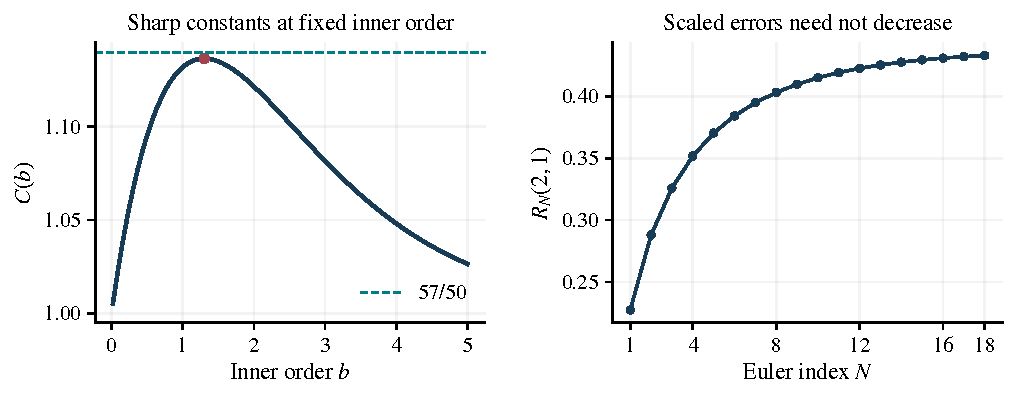
\includegraphics[width=\textwidth]{figures/euler_constants.pdf}
\caption{Left: the inner-order constant $C(b)$ and its unique maximum,
with the convenient rational budget $57/50$. Right: a finite diagnostic
plot of the scaled errors $R_N(2,1)$. Its initial increase is certified
symbolically by Proposition~\ref{prop:scaled-error-counterexample}; the
plot is not used to prove a global shape or to identify its eventual
maximum. The curves are numerical illustrations of proved bounds.}
\label{fig:euler}
\end{figure}

\begin{figure}[htbp]
\centering
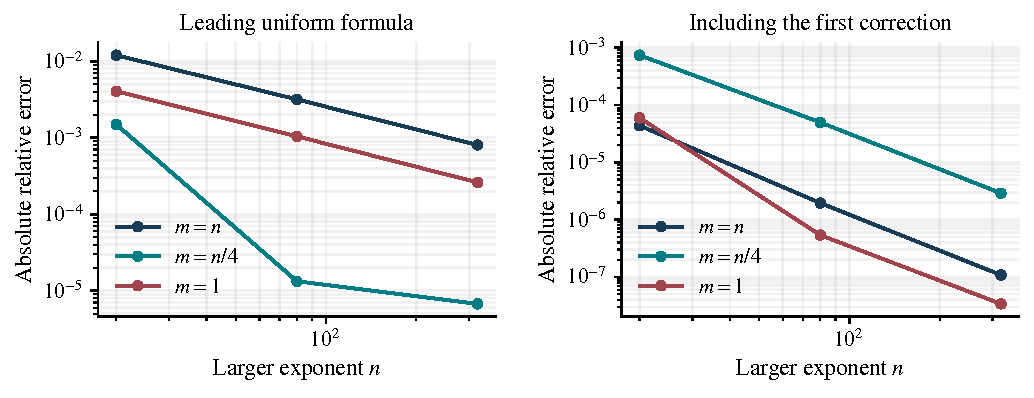
\includegraphics[width=\textwidth]{figures/uniform_moment_errors.pdf}
\caption{Absolute relative errors in the all-ratio moment approximation,
before and after the first correction, for three of the seven tested
parameter families. The reference values are computed by quadrature in
$t=-\log x$, independent of the inverse-coordinate saddle construction.
The first correction generally improves accuracy at sufficiently large
exponents; cancellation can make an uncorrected finite case unusually
accurate, so pointwise improvement at every input is not a theorem.}
\label{fig:moments}
\end{figure}

For example, for $m=n=20,80,320$, the corrected relative errors have
absolute values approximately
$4.39\times10^{-5}$, $1.95\times10^{-6}$, and $1.08\times10^{-7}$.
For $m=n/4$ the corresponding values are approximately
$7.41\times10^{-4}$, $4.98\times10^{-5}$, and $2.89\times10^{-6}$.
These finite values illustrate the theorem but cannot determine the
uniform error constant. The axis diagnostic also checks against the
source's strict factorial comparison; it does not incorrectly substitute
$M_{n,0}=\Gamma(n+1)$ as an exact identity.

\begin{figure}[htbp]
\centering
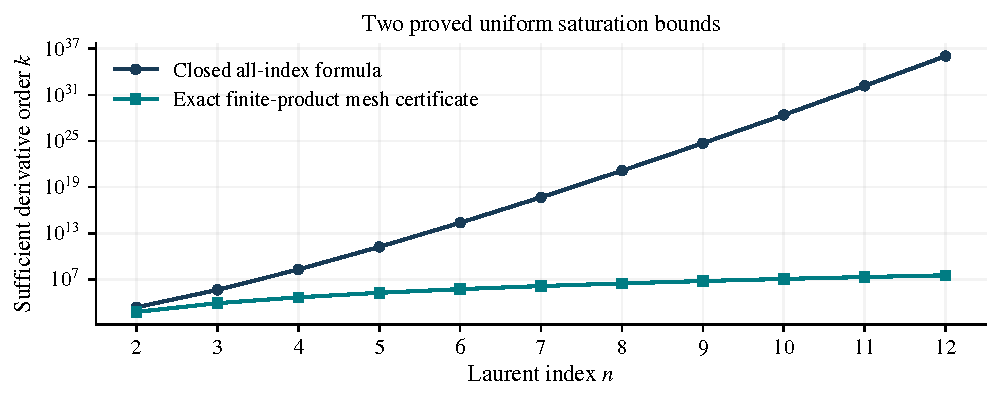
\includegraphics[width=0.86\textwidth]{figures/lerch_thresholds.pdf}
\caption{Two sufficient Lerch saturation thresholds: the explicit
all-index formula and the improved bounds obtained from exact finite
Sturm isolation of $B_n$. The vertical axis is logarithmic. The displayed
integers are consequences of the same proved sign-transfer criterion;
they are not estimates of the sharp transition. In particular the known
index-two threshold is $1$, below both curves.}
\label{fig:lerch}
\end{figure}

\subsection{A portable replay protocol}

The archive provides \code{code/verify_all.py}. The default command
runs the exact certificates and finite matrix audit. It records commands,
exit status, elapsed time, and output hashes in a replay manifest. A
\code{--numerical} option additionally recomputes the 24 moment diagnostics;
the independent 120-digit Mellin audit has its own optional command.
No verification command requires network access or a checkout of the
source repository. The inherited gamma-slope program is copied unchanged
and explicitly attributed.

The Gaussian input is \code{code/gaussian/gaussian_candidates.json}.
The historical discovery files retain both the unsuccessful first
weight-thirteen search and the successful higher-precision search.
Their role is audit history; the verifier reads only the canonical
retained/rejected records. This avoids inadvertently promoting an obsolete
integer vector when integrating the work.

LaTeX compilation uses \code{code/build_article.py} to concatenate the
preamble, ordered section fragments and bibliography into a complete
\code{article.tex}, then \code{latexmk -pdf article.tex}. The final
article source can be compiled without Python when the bundled figure
PDFs are present. Figure regeneration is optional and uses the saved
diagnostic data. The archive includes a file-hash manifest and the exact
source revision for every inherited dependency.

\FloatBarrier

% ===== sections/08_research_agenda.tex =====
\section{Further research questions and a proposed programme}
\label{sec:agenda}

The strongest next steps are those that convert the new structural
information into a sharper theorem or a finite exact identity
certificate. The following questions are separated by their mathematical
obstruction and the kind of evidence that would count as progress.

\subsection{Sharp fixed-pair Euler errors}

For fixed $a,b>0$, determine
\[
 C(a,b)=\max_{N\ge1}R_N(a,b)
\]
and the set of maximizing indices. Existence follows from positivity and
$R_N\to0$, but the maximizer can occur after the first remainder.
Does the sequence have at most one local maximum outside the parameter
regions where monotonicity is already proved? Are there curves in the
$(a,b)$ plane across which the maximizing integer changes? A useful
first goal is an analytic classification of the sign of $R_{N+1}-R_N$
using the two-variable positive probability kernel.

The limit $a\downarrow0$ at fixed $b$ gives $C(a,b)\to C(b)$ by the
first-index lower bound and the uniform upper bound. Determine
a uniform first correction in $a$, and whether the maximizing index is
eventually $1$ on compact $b$ intervals. Joint limits where $a$ or $b$
approach zero while $N$ grows may reveal additional transition scales.
They cannot be inferred from the fixed-pair limit $R_N\to0$ alone.

The scalar proof suggests a broader approximation problem: characterize
families $f$ whose fixed-midpoint divided differences are monotone and
whose endpoint secants yield optimal multiplicative-increment bounds.
For Euler-type transformations, this could produce universal constants
for positive kernels beyond the harmonic double polylogarithms.

\subsection{Effective all-ratio moment asymptotics}

The theorem proves the existence of a remainder constant for each fixed
order. Produce explicit numerical constants valid for all $0\le m\le n$
above a stated $n_0$. This requires quantitative bounds on the normalized
phase and amplitude derivatives, plus the global phase-gap constant.
The existing interval proof of the slope inequality provides a concrete
starting point rather than an abstract compactness argument.

Can the inherited monotonicity of $J$ be proved by a short analytic
inequality, eliminating the compact interval computation? Ordinary
convexity of $\log\Gamma$ is insufficient, as the source already explains.
A successful proof would make the all-ratio theorem fully analytic and
could sharpen its uniform curvature bounds.

Find a uniform approximation retaining the exponentially small
fixed-$m$ corrections while also handling the balanced region. The
current theorem controls every algebraic order, but matching it to the
residue expansion requires analysis of the correction
$q(y)e^y/\gamma-1$ when $m e^{-s}$ changes scale. One target is an
explicit overlap theorem that recovers both expansions with their own
natural error budgets.

The probabilistic corollary invites quantitative questions. Establish a
uniform Kolmogorov or total-variation error bound for
$\sqrt H(Y-s)$, then a uniform Edgeworth expansion with tail control.
The metric, centering and normalization must be fixed before a rate is
claimed. Related questions concern logarithmic derivatives of $M_{n,m}$,
which encode the mean and covariance of $\log f(x)$ and $\log f(1-x)$
under the tilted moment measure.

\subsection{Appell mesh, saturation, and growing zero configurations}

The bound $\operatorname{mesh}(Q_n)\ge(3n)^{-(n-2)}$ is deliberately
coarse. Determine the actual asymptotic size of the smallest gap. Even a
polynomial lower bound $\operatorname{mesh}(Q_n)\gg n^{-A}$ would, through
the proved transfer argument, give a polynomial sufficient threshold
$k\gg n^{2A+2}$. Such an improvement would extend the growing-index regime
far beyond $n=O(\log k/\log\log k)$.

The current proof estimates the product over roots by its worst distance
to any root. Replace that bound with local reciprocal-gap sums such as
\[
 \sum_{\ell\ne j}|x_{n,j}-x_{n,\ell}|^{-1}
 \quad\hbox{and}\quad
 \sum_{\ell\ne j}|x_{n,j}-x_{n,\ell}|^{-2}.
\]
Together with centered gamma moments, this may improve the location
error $O(n/\sqrt{k})$ and recover constant offsets uniformly for growing
$n$. It would also distinguish extreme roots from interior roots when
their local geometries differ.

For each small index, determine the least $k$ that guarantees saturation
for every $\rho\in[0,1]$, and the least $k$ for each global motion law.
Certified continuation, exact endpoint analysis and the global
multiplicity bound should be used together. The new terminal-branch
theorem settles its direction whenever that branch is simple, but it
does not order the motion of all interior branches at small $k$.

More generally, replace $W_\rho$ by a positive family with a uniformly
bounded logarithmic derivative. The sign-transfer proof then changes
only through that bound. Determine which non-Lerch deformations inherit
effective saturation, and which require additional endpoint integrability.
This would isolate the root-stability mechanism from its original
special-function setting.

\subsection{Integral presentations and exact Gaussian identities}

The immediate identity target remains a finite rational certificate for
the existing $S_6$ formula. Use the integral shuffle diagonalization to
remove redundant coordinates before building Cayley, distribution,
conjugation and regularized double-shuffle rows. Each regularized row
must carry an analytic justification. A successful computation should
return an exact row combination producing the target, not only a rank
or a floating-point null vector.

\begin{conjecture}[A uniform Gaussian span question]
\label{conj:uniform-span}
For every integer $m\ge1$, the number
$S_{2m}+2\beta(2m)\log2$ belongs to the rational span of
\[
 \{g_{2m-2j,\,2j+1}:0\le j<m\}
 \cup\{\pi^{2m+1}\}
 \cup\{\beta(2j)\zeta(2m+1-2j):1\le j<m\}.
\]
\end{conjecture}

The proved $S_2,S_4$ cases in the repository and the conjectural
$S_6,S_8,S_{10},S_{12}$ relations motivate this formulation. Their
different evidential status is essential. The all-weight matrix theorem
justifies the chosen coordinates but does not prove that a mixed sum
belongs to their span. An appropriate generating-function identity could
settle many weights at once; until it is found, exact certificates at
successive weights are meaningful intermediate goals.

Determine analogous integral diagonal forms at even weights, other roots
of unity, and greater depth. The odd-weight proof uses the reflection
$y\leftrightarrow1-y$ and central factorials in a precise way; it does
not automatically furnish a higher-depth presentation. Integral data
would identify torsion primes and optimal denominator budgets before
expensive exact linear algebra is attempted.

\subsection{A practical order of attack}

The nearest finite targets are the $S_6$ row certificate, sharper
certified Appell mesh bounds, and explicit constants in the first-order
all-ratio moment error. The more structural targets are an analytic
global slope proof, a general mixed-Gaussian generating identity, and
an asymptotic theory for the Appell mesh. These tasks can proceed in
parallel because their proof dependencies are largely separate.

For every proposed identity, freeze the basis and integer vector before
validation; recompute it by an independent representation; produce exact
residual bounds; and pursue an algebraic or analytic certificate of
equality. For every asymptotic claim, state all joint parameter ranges
and preserve the distinction between finite diagnostics and a uniform
remainder proof. The present package supplies examples of both successful
proofs and a rigorously rejected numerical candidate.

% ===== sections/09_provenance.tex =====
\appendix
\section{Source provenance and integration map}
\label{app:provenance}

All comparisons to the repository refer to commit
\begin{center}\sourcecommit\end{center}
in \url{https://github.com/VladimirReshetnikov/ProveIt}.
The commit is dated 10 October 2026 and publishes the reviewed
375-page real-order manuscript milestone. The present article is a
separate continuation prepared against that version. The archive's
\code{provenance.json} records hashes of the relevant original files,
the inherited verifier, and the provenance of each main claim.

\begin{longtable}{@{}P{0.28\textwidth}P{0.40\textwidth}P{0.26\textwidth}@{}}
\toprule
New section & Suggested manuscript location & Status update\\
\midrule
\endhead
Sharp universal Euler bound & After the real-order Euler and Gaussian
axis analysis in Chapter 5. & Close the universal-constant question;
retain stronger restricted bounds.\\
All-ratio moments & After Chapter 7, together with the companion report's joint-moment and
certified proportional saddle material. & Add an unrestricted-ratio algebraic
expansion; retain fixed-order exponential results.\\
Effective Lerch zeros & After the global variation bound and fixed-index
concentration material in Chapter 9. & Replace a purely existential
threshold by an explicit sufficient one; add the growing-index regime.\\
Integral shuffle minor & With the Gaussian reduction and relation-matrix
material in Chapters 4--5. & Add the integral presentation and denominator
theorem with the Zagier/Ma attribution.\\
$S_{10}$ and $S_{12}$ & Alongside the frozen $S_6$ and $S_8$ candidates. &
Mark both as conjectural; attach exact proximity certificates.\\
Research agenda & Revise the corresponding open items in Chapter 10. &
Keep fixed-pair constants, sharp thresholds and mixed reductions open.\\
\bottomrule
\end{longtable}

The inherited global-slope theorem is sourced from the report
\code{uniform-transition-continuation}, in its section file
\code{sections/04b-proportional-moments.tex}.
An unchanged copy is included as \code{integration/inherited_global_slope.tex},
and its original exact verifier is included under \code{code/moments/}.
The original file includes its endpoint argument, compact certificate,
and proportional theorem. It is reference material, not a second new
proof or a required input to compiling this article.

For an explicit view of that dependency, write $P=\psi_1$ and
\[
 \frac{J'}J=
 \frac{F(x)}{f(x)}+\frac{F(1-x)}{f(1-x)}
 -\frac{P(x)}{F(x)}-\frac{P(1-x)}{F(1-x)}.
\]
The source bounds this expression below by $176/225$ on
$(0,1/16]$ using convergent gamma series and elementary inequalities;
reflection handles $[15/16,1)$. Its 256 rational intervals cover
$[1/16,1/2]$ completely. The replayed minimum lower endpoint is
\[
 \frac{2237344070433247164830307425599}
      {1267650600228229401496703205376}>\frac74.
\]
Every rounding is outward on a $2^{-100}$ grid, and all special constants
are enclosed by rational sums with explicit tails. Thus this inherited
input is a computer-assisted theorem with a portable exact replay,
not a sampled monotonicity assertion.

The supplied integration notes include exact replacement wording for
the superseded Euler caution and the research-status entries. They do
not propose removing the original hypotheses or recasting a numerical
period relation as a proved identity. No change to the remote repository
is part of this deliverable; the modular sections and complete source
are ready for review and integration.

\begin{thebibliography}{99}

\bibitem{repo}
V.~Reshetnikov and contributors,
\emph{ProveIt: Polylogarithms manuscript and continuation reports},
repository revision \sourcecommit, 10 October 2026.
\url{https://github.com/VladimirReshetnikov/ProveIt/tree/3447bc59b78d138a7f0d536b66ac6e5cc5d5e49f/Analysis/Polylogarithms/docs/manuscript}.
The exact inherited dependencies are identified in Appendix~\ref{app:provenance}
and in the accompanying provenance record.

\bibitem{Amdeberhan}
T.~Amdeberhan, M.~W.~Coffey, O.~Espinosa, C.~Koutschan,
D.~V.~Manna, and V.~H.~Moll,
\emph{Integrals of powers of loggamma},
Proceedings of the American Mathematical Society \textbf{139} (2011),
no.~2, 535--545.
\href{https://doi.org/10.1090/S0002-9939-2010-10589-0}{doi:10.1090/S0002-9939-2010-10589-0}.
Author preprint:
\url{https://www.math.tulane.edu/~vhm/papers_html/lg-subm.pdf}.

\bibitem{Bailey}
D.~H.~Bailey, D.~Borwein, and J.~M.~Borwein,
\emph{On Eulerian log-gamma integrals and Tornheim--Witten zeta functions},
The Ramanujan Journal \textbf{36} (2015), nos.~1--2, 43--68.
\href{https://doi.org/10.1007/s11139-012-9427-1}{doi:10.1007/s11139-012-9427-1}.
Author copy dated 28 July 2012:
\url{https://www.davidhbailey.com/dhbpapers/log-gamma.pdf}.

\bibitem{DLMFLaplace}
NIST Digital Library of Mathematical Functions,
\emph{Section 2.3: Integrals of a Real Variable}, particularly
Section 2.3(iii), Laplace's method. Accessed 10 October 2026.
\url{https://dlmf.nist.gov/2.3}.

\bibitem{DLMFGamma}
NIST Digital Library of Mathematical Functions,
\emph{Section 5.7: Series Expansions}, gamma and logarithmic-gamma
series. Accessed 10 October 2026.
\url{https://dlmf.nist.gov/5.7}.

\bibitem{efflerch:BKS}
P.~Br\"and\'en, I.~Krasikov, and B.~Shapiro,
\emph{Elements of P\'olya--Schur theory in the finite difference setting},
Proceedings of the American Mathematical Society \textbf{144} (2016),
4831--4843. Theorem~1 records the classical Riesz mesh-preservation theorem.
\href{https://doi.org/10.1090/proc/13115}{doi:10.1090/proc/13115}.
Author-hosted full text:
\url{https://staff.math.su.se/shapiro/Articles/FiniteDifference.pdf}.

\bibitem{Zagier}
D.~Zagier,
\emph{Evaluation of the multiple zeta values
$\zeta(2,\ldots,2,3,2,\ldots,2)$},
Annals of Mathematics \textbf{175} (2012), 977--1000.
Section~5, equations (36)--(37).
\href{https://doi.org/10.4007/annals.2012.175.2.11}{doi:10.4007/annals.2012.175.2.11}.
\url{https://annals.math.princeton.edu/wp-content/uploads/annals-v175-n2-p11-p.pdf}.

\bibitem{Ma}
D.~Ma,
\emph{Inverse of a matrix related to double zeta values of odd weight},
2015. \href{https://arxiv.org/abs/1510.06094}{arXiv:1510.06094}.

\bibitem{MaTeo}
Y.~Ma and L.-P.~Teo,
\emph{Another Proof of Zagier's Matrix Conjecture},
Journal of Integer Sequences \textbf{25} (2022), Article 22.6.4.
\url{https://cs.uwaterloo.ca/journals/JIS/VOL25/Teo/teo4.pdf}.

\end{thebibliography}

\end{document}
